\RequirePackage{amsmath}
\documentclass[envcountsame,runningheads,a4paper]{llncs}

\usepackage{cmap}
\usepackage{makeidx}
\usepackage{breakurl}
\usepackage{underscore}

\usepackage[english]{babel}
\usepackage[utf8x]{inputenc}
\usepackage[T1]{fontenc}
%\usepackage{a4wide}
%\usepackage{enumerate}
\usepackage{paralist}
%\usepackage{palatino}
\usepackage[usenames, dvipsnames]{color}
\usepackage{hyperref}
\usepackage{multicol}
\usepackage{verbatim}
\usepackage{cite}


\usepackage{amssymb,amsfonts,mathrsfs}
\usepackage{stmaryrd}
\usepackage{marvosym}
\usepackage{bussproofs}

%\usepackage[left=2cm,right=2cm]{geometry}

\usepackage{tikz}
\usetikzlibrary{arrows,positioning,decorations.pathreplacing,automata,shadows}
\usepackage{tikz-cd}

%\usepackage{parskip}
%\usepackage{\parintent}{15pt}


%%%%%%%%%%%%%%%%%%%%%%%%%%%%%%%%%%%%%%%%
%                                      %
%         Commandes persos             %
%                                      %
%%%%%%%%%%%%%%%%%%%%%%%%%%%%%%%%%%%%%%%%

% Syntax 
\newcommand{\Nat}{\textnormal{Nat}}
\newcommand{\Tree}{\textnormal{Tree}}
\newcommand{\Succ}{\operatorname{S}}
\newcommand{\Zero}{\textnormal{Z}}
\newcommand{\Fix}{\operatorname{fix}}
\newcommand{\Unroll}{\operatorname{unroll}}
\newcommand{\Pos}{\operatorname{Pos}}
\newcommand{\In}{\operatorname{in}}
\newcommand{\Inr}{\operatorname{inl}}
\newcommand{\Inl}{\operatorname{inr}}
\newcommand{\Out}{\operatorname{out}}
\newcommand{\Ret}{\operatorname{return}}
\newcommand{\Bind}[3]{\operatorname{let} #2 \Leftarrow #1 \operatorname{in} #3}
\newcommand{\lcase}[3]{\operatorname{case} #1 \operatorname{of} \, \Zero \Rightarrow #2; \Succ(x) \Rightarrow #3}
\newcommand{\scase}[3]{\operatorname{case} #1 \operatorname{of} \, \Inl(x) \Rightarrow #2; \Inr (x) \Rightarrow #3}
\newcommand{\pcase}[2]{\operatorname{case} #1 \operatorname{of} \, (x,y) \Rightarrow #2}

% Arrows 
\makeatletter
\newcommand\twoheaduparrow{%
\mathrel{\mathchoice
  {\raise2pt\hbox{%
  \ooalign{\hss$\uparrow$\hss\cr\lower2pt\hbox{%
  $\uparrow$}}}}
  {\raise2pt\hbox{%
  \ooalign{\hss$\uparrow$\hss\cr\lower2pt\hbox{%
  $\uparrow$}}}}
  {\raise1.5pt\hbox{%
  \ooalign{\hss$\scriptstyle\uparrow$\hss\cr\lower1.5pt\hbox{%
  $\scriptstyle\uparrow$}}}}
  {\raise1.1pt\hbox{%
  \ooalign{\hss$\scriptscriptstyle\uparrow$\hss\cr\lower1.1pt\hbox{%
  $\scriptscriptstyle\uparrow$}}}}
}}
\makeatletter
\newcommand\twoheaddownarrow{%
\mathrel{\mathchoice
  {\raise2pt\hbox{%
  \ooalign{\hss$\downarrow$\hss\cr\lower2pt\hbox{%
  $\downarrow$}}}}
  {\raise2pt\hbox{%
  \ooalign{\hss$\downarrow$\hss\cr\lower2pt\hbox{%
  $\downarrow$}}}}
  {\raise1.5pt\hbox{%
  \ooalign{\hss$\scriptstyle\downarrow$\hss\cr\lower1.5pt\hbox{%
  $\scriptstyle\downarrow$}}}}
  {\raise1.1pt\hbox{%
  \ooalign{\hss$\scriptscriptstyle\downarrow$\hss\cr\lower1.1pt\hbox{%
  $\scriptscriptstyle\downarrow$}}}}
}}


% Results
\newcommand{\res}{\operatorname{results}}

% Effects 
\newcommand{\prEff}{\operatorname{pr}}
\newcommand{\orEff}{\operatorname{or}}
\newcommand{\exEff}{\operatorname{raise}}

% Reduction
\newcommand{\reduces}{\rightarrowtail}
\newcommand{\reductionPair}[2]{#1 \leadsto #2}
\newcommand{\sqeq}{\sqsubseteq}


% Mixed non-determinism
\newcommand{\drop}{\operatorname{drop}}
\newcommand{\odd}{\operatorname{odd}}
\newcommand{\even}{\operatorname{even}}


%%%%% ---- THEOREMS ----- 

\newenvironment{atheorem}[1][]{\begin{theorem}[#1]}{\end{theorem}}
\newenvironment{alemma}[1][]{\begin{lemma}[#1]}{\end{lemma}}
\newenvironment{acorollary}[1][]{\begin{corollary}[#1]}{\end{corollary}}
\newenvironment{adefinition}[1][]{\begin{definition}[#1]\em}{\end{definition}}


% Hide-if-not-ENS
\newenvironment{ensps}
{ } 
{ }
%{ \rule{1ex}{1ex} }
%{ \rule{1ex}{1ex} }
%{ \comment} 
%{ \endcomment }

\title{Contextual equivalence for algebraic effects under call-by-value, with combined  probability and nondeterminism as a worked example}
\author{Aliaume Lopez\inst{1} 
  \and Alex Simpson \inst{2}}
\institute{École Normale Supérieure Paris-Saclay,
    \\ Université Paris-Saclay, France \\ \email{aliaume.lopez@ens-paris-saclay.fr} \\ \;  \and
    Faculty of Mathematics and Physics \\ University of Ljubljana, Slovenia \\ \email{Alex.Simpson@fmf.uni-lj.si} }
%
\titlerunning{Contextual equivalence, algebraic effects, probability and nondeterminism}
\authorrunning{A.\ Lopez and A.\ Simpson}

%\providecommand{\event}{Fossacs 2018} 


\begin{document}

\maketitle

\begin{abstract} 
We present a systematic study of contextual equivalence
in the presence of algebraic effects, adapting previous work of Johann, Simpson and Voigtl\"{a}nder
from its original call-by-name setting to call-by-value. As in the previous work, the central idea is to specify a
basic operational preorder on ground-type effect trees. We consider three main approaches to 
defining such preorders: using direct operational considerations, 
via denotational semantics, and via (in)equational axiomatisations. To illustrate the utility of our methodology, we present a nontrivial case study: the combination of probabilistic choice with (either angelic or demonic) nondeterminism. In this case, the three methods of specifying the basic preorder (operationally in terms of Markov decision processes, denotationally using  a suitable powerdomain, and axiomatically) all lead to the same contextual equivalence.
%in the continuation of preexisting work \cite{gom}. To reach 
%this objective, we extend a call-by-value PCF with a signature of algebraic effects, 
%and give an abstract equality between the contextual equivalence for this language and a
%usable logical relation, independently of the signature itself. Generic meta
%theorems are then proven using this abstract equivalence. To justify the
%usefulness of this approach, a direct link with denotational semantics
%and the work of Plotkin and Power \cite{plotkin2001adequacy} is
%developed, and signature of mixed non-determinism and probabilities is studied
%in-depth.
\end{abstract}


%\newpage

\section{Introduction}

Contextual equivalence in the style of Morris
has imposed itself as a very simple and powerful
way to express what an equivalence on programs should be. 
However
this operational notion of equivalence is rarely usable 
as-is \cite{pitts1997operationally}.

For this reason, many other forms of equivalences have 
been developed in the past years: bisimulations 
and their refinements (environmental bisimulations, 
bisimulations up-to) \cite{koutavas2011applicative}, 
game semantics \cite{abramsky1999game}, 
denotational interpretation in domains \cite{scott1982domains}, 
higher order logic on 
programs \cite{honda2005observationally} 
and logical relations \cite{Pitts2000}.

Unsurprisingly one can observe extreme variations on 
the complexity of such methods when changing  
the class of effects studied. This has to do with 
the fact that most of the operational semantics 
are deeply tied with the effects of the language, 
and adding or removing effects changes the overall 
shape of the semantics. For denotational interpretation,
the problem is less visible because it is transposed 
into domain theoretic constructions, such as powerdomains, distributive laws,
and solving domain equations.

To be able to give uniform results, the first 
step is to restrict the class of effects
to \emph{algebraic} ones, 
allowing to separate the semantics 
of the effects from the semantics of the ground language
itself by using computation trees \cite{plotkin2001adequacy}.

Following the work done by Patricia
Johann, Alex Simpson and Janis Voigtländer \cite{gom}, we then define 
a logical relation to capture the contextual 
equivalence, and apply this result to a wide class of known effects 
such as: non-determinism, probabilities, input-output, and exceptions. 
The main difference is that our approach 
is done in a call-by-value setting, as opposed 
to call-by-name.


We also continue the work done by Plotkin and Power \cite{plotkin2001adequacy}
by using their result to link our setting to the denotational approach. This 
should be considered as an empirical proof of the usefulness of this method. 
Continuing in this direction, we study a concrete example combining
non-determinism and probability, a subject that has been regularly encountered 
in denotational models \cite{tix2009semantic} \cite{JGL-mscs16}
\cite{KeimelP2016} and the study concurrent programs
\cite{Mislove2000} \cite{mislove2004axioms}.


%\newpage

\section{Parametrized class of languages}

The studied class of languages is based on PCF \cite{plotkin1977lcf} in a call-by-value setting 
parametrized by extra operations called \emph{effects}, which is a setting very similar to 
the one studied by Plotikn and Power \cite{plotkin2001adequacy}. 
The main motivation is to find result similar to the ones 
we already have in a call-by-name setting \cite{gom}.

The parameter for this class of languages is $\Sigma$,  
a set of symbols with a finite arity.
Refined call-by-value \cite{Ugo2017} is used instead of regular call-by-value 
to help separating effect evaluation and regular term 
evaluation in the language. However the results apply equally to both 
languages because there is a direct translation from one to
the other that can be seen in Figure \ref{fig:refinedNormal}.

The type system is fairly simple, with only 
natural numbers and functions from one 
type to another type as it can be seen in Figure \ref{fig:language}.
The type inference rules for this language can be seen in Figure
\ref{fig:inference:typing}, no rule should be surprising
but it is worth mentioning that already the inference 
rules are making a distinction between \emph{computations}
and \emph{values}.

This setting is purposely restricted, and several improvements can 
be added without technical issue. For instance, more complex types 
such as sum, products and even type polymorphism can be studied 
in this context. In fact, logical relations excel in proving parametricity 
results \cite{wadler1989theorems}.
In the spirit of simplicity 
and to allow comparison with the work on bisimulations by
Ugo Dal Lago, Francesco Gavazzo and Paul Blain Lévi 
\cite{Ugo2017} we take the same kind of effect signature 
as they do. Technically, it means that compared to 
the paper from Johann et al. \cite{gom} it lacks 
three of the four effect constructions, but as noticed 
in the said paper, all of the constructions share the
same pattern of proof, so that they actually treated 
only one of the four cases in their proofs.


\begin{figure}[h!]
    \begin{align*}
        \tau :=& ~\Nat ~|~ \tau \to \tau \\
        V :=& ~x ~|~ \lambda x:\tau. M ~|~ \Zero ~|~ \Succ V \\
        M :=& ~\Ret V ~|~ V V ~|~ \Fix V \\
                    &|~ \lcase{V}{M}{M} \\
                    &|~ \Bind{M}{x:\tau}{M} \\
                    &|~ \sigma(\underbrace{M, \dots, M}_n ) \quad \text{ where } (\sigma,n)  \in \Sigma
    \end{align*}
    \caption{Refined Call-By-Value PCF with effects}
    \label{fig:language}
\end{figure}

\begin{figure}[h!]
    \begin{equation*}
        \begin{array}{rl}
            (\lambda x:\tau. N)M &\leftarrow \Bind{M}{x:\tau}{N} \\
            M N &\rightarrow \Bind{M}{f:\sigma \to \tau}{\Bind{N}{x:\sigma}{ f x }} 
        \end{array}
    \end{equation*}
    \caption{Translation between refined and regular call-by-value}
    \label{fig:refinedNormal}
\end{figure}


\begin{figure}[h]
    \begin{center}
        % Identity on variables 
            \AxiomC{}
            \UnaryInfC{$\Gamma, x:\tau \vdash_V x : \tau$}
            \DisplayProof 
        \hskip 1.5em
        % Return a value 
            \AxiomC{$\Gamma \vdash_V V : \tau$}
            \UnaryInfC{$\Gamma \vdash_C \Ret V : \tau$}
            \DisplayProof 
        \hskip 1.5em
        % Lambda abstraction 
            \AxiomC{$\Gamma, x : \tau \vdash_C M : \tau'$}
            \UnaryInfC{$\Gamma \vdash_V \lambda x:\tau. M : \tau \to \tau'$}
            \DisplayProof 
        \hskip 1.5em
        % Zero 
            \AxiomC{}
            \UnaryInfC{$\Gamma \vdash_V \Zero : \Nat$}
            \DisplayProof
        \hskip 1.5em
        \vskip 1em
        % Succ 
            \AxiomC{$\Gamma \vdash_V V : \Nat$}
            \UnaryInfC{$\Gamma \vdash_V \Succ V : \Nat$}
            \DisplayProof
        \hskip 1.5em
        % Fixed point 
            \AxiomC{$\Gamma \vdash_V V : (\tau \to \tau') \to \tau \to \tau'$}
            \UnaryInfC{$\Gamma \vdash_C \Fix V : \tau \to \tau'$}
            \DisplayProof
        \hskip 1.5em
        % Application  
            \AxiomC{$\Gamma \vdash_V V : \tau \to \tau'$} 
            \AxiomC{$\Gamma \vdash_V W : \tau$}
            \BinaryInfC{$\Gamma \vdash_C V W : \tau'$}
            \DisplayProof
        \hskip 1.5em
        \vskip 1em
        % Case   
            \AxiomC{$\Gamma \vdash_V V : \Nat$} 
            \AxiomC{$\Gamma \vdash_C M_1 : \tau$}
            \AxiomC{$\Gamma, x:\Nat \vdash_C M_2 : \tau$}
            \TrinaryInfC{$\Gamma \vdash_C \lcase{V}{M_1}{M_2} : \tau$}
            \DisplayProof
        \hskip 1.5em
        % Bind 
            \AxiomC{$\Gamma \vdash_C M : \tau$} 
            \AxiomC{$\Gamma, x:\tau \vdash_C N : \tau'$}
            \BinaryInfC{$\Gamma \vdash_C \Bind{M}{x:\tau}{N} : \tau'$}
            \DisplayProof
        \hskip 1.5em
        \vskip 1em
        % Effect 
            \AxiomC{$(\sigma,n) \in \Sigma$}
            \AxiomC{$\forall 1 \leq i \leq n, \quad \Gamma \vdash_C M_i : \tau$}
            \BinaryInfC{$\Gamma \vdash_C \sigma(M_1, \dots, M_n) : \tau$}
            \DisplayProof
    \end{center}
    \caption{Inference rules for typing}
    \label{fig:inference:typing}
\end{figure}


\begin{example}[Signature for combined probabilities and non-determinism]
    In the case of combining non-determinism and probabilities, one can
    consider a fair coin toss $\prEff$ of arity two, with a demonic 
    choice operator $\orEff$ of arity two. The signature of the language 
    is therefore $\Sigma = \{ (\prEff,2), (\orEff,2) \}$.
\end{example}


It can be shown that the set of values of type $\Nat$ is isomorphic to $\mathbb{N}$
and therefore we will identify the two sets using $\underline{n}$ to denote 
the value corresponding to $n$.


%\newpage

\subsection{Uniform Small-Step Semantics}

The first step to define contextual equivalence 
is to define an operational semantics.
Because we are considering a \emph{class} of languages 
we are going to have a two steps approach: first 
interpret the core language independently of the parameter $\Sigma$
and only then \emph{refine} this semantics to give one to the effects.

A small-step semantics is given using 
stack and frames \cite{gom}.
The link between this small-step semantics 
and its big-step counterpart is 
made both in \cite{plotkin2001adequacy} 
and in \cite{Pitts2000}. This method
can be traced back to \cite{Amadio2008} (1998) page 184 and 
\cite{Felleisen1992}.

In a refined call-by-value calculus stacks and frames 
are very simple as it can be seen in Figure \ref{fig:stacks:frames}, 
but few cases does not imply little expressive power, and 
in fact any term with one free variable can be turned into 
a stack. A type system for stacks is also defined Figure \ref{fig:stacks:types}.

\begin{figure}[h]
    \begin{center}
        \begin{align*}
            E &:= \Bind{\square}{x:\tau}{M} \\
            S &:= Id ~|~ S \circ E
        \end{align*}
    \end{center}
    \caption{Stacks and Frames}
    \label{fig:stacks:frames}
\end{figure}


\begin{figure}[h]
    \begin{center}
        \AxiomC{$x:\tau \vdash_C M : \tau'$}
        \UnaryInfC{$\vdash \Bind{\square}{x:\tau}{M} : 
            \tau \multimap \tau'$}
        \DisplayProof
        \hskip 1.5em
        \AxiomC{$\vdash E : \tau \multimap \tau'$}
        \AxiomC{$\vdash S : \tau' \multimap \tau''$}
        \BinaryInfC{$\vdash S \circ E : \tau \multimap \tau''$}
        \DisplayProof
        \vskip 1.5em
        \AxiomC{}
        \UnaryInfC{$\vdash Id : \tau \multimap \tau$}
        \DisplayProof
    \end{center}
    \caption{Typing of Stacks and Frames}
    \label{fig:stacks:types}
\end{figure}


Because stacks are just a \texttt{let}-binding with one hole, we can define 
application of a stack to a \emph{computation} which returns a computation
obtained by substitution as defined in Figure \ref{fig:stackapplication}.

\begin{figure}[h]
    \begin{align*}
        Id\{ M \} &= M \\
        (S \circ E) \{ M \} &= S \{ E \{ M \} \} \\
        (\Bind{\square}{x : \tau}{N} \{ M \}) &= \Bind{M}{x : \tau}{N}
    \end{align*}
    \caption{Stack application}
    \label{fig:stackapplication}
\end{figure}

%\begin{adefinition}[Stack application]
    %Given a stack $S$ and a computation term $M$
    %we can define $S\{M\}$ to be the application 
    %of the stack to the term by induction on $S$
    %following the rules in Figure \ref{fig:stackapplication}.
%\end{adefinition}

We say that a pair $(S,M)$ of a stack and a term is well 
typed when $S : \sigma \multimap \tau$ and $M : \sigma$, 
this will be consistent with the following safety theorem.

\begin{alemma}[Safety]
    Typing of stacks and frame is coherent
    with the typing of terms and stack application.

    \begin{equation*}
        \vdash S : \tau \multimap \tau' \, \wedge \, 
        \vdash_C M : \tau
        \implies
        \vdash_C S\{M\} : \tau'
    \end{equation*}
\end{alemma}

Now that evaluation stacks are defined, we can use them to define 
the operational semantics of our language. First of all, on 
simple computations, we can define a term reduction 
as in Figure \ref{fig:termred}, then given this basic 
reduction, we can use stacks to generalise the evaluation 
process to more terms as seen in Figure \ref{fig:evalstep}.


\begin{figure}[h]
    \begin{center}
        \begin{equation*}
            \begin{array}{lcl}
                (\lambda x:\tau. M) V & \leadsto & M[x := V] \\
                \lcase{\Zero}{M_1}{M_2} & \leadsto & M_1 \\
                \lcase{\Succ(V)}{M_1}{M_2} & \leadsto & M_2[x := V] \\
                \Bind{\Ret V}{x : \tau}{M} & \leadsto & M[x := V] \\
                \Fix V & \leadsto & V (\lambda x. \Bind{(\Fix V)}{g}{g x})
            \end{array}
        \end{equation*}
    \end{center}
    \caption{Term reduction}
    \label{fig:termred}
\end{figure}


\begin{figure}[h]
    \begin{center}
        \begin{equation*}
            \begin{array}{lclr}
                (S,E\{M\}) & \reduces & (S \circ E, M) \\
                (S \circ E, \Ret V) & \reduces & (S, E \{ \Ret V \}) \\
                (S,M) & \reduces & (S,M') & \text{ when } M \leadsto M'
            \end{array}
        \end{equation*}
    \end{center}
    \caption{Evaluation steps}
    \label{fig:evalstep}
\end{figure}

\begin{alemma}[Safety]
    If a pair $(S,M)$ is well-typed then 
    evaluation preserves this property 
    and the co-domain of the stack never changes.
\end{alemma}

\begin{example}[Reduction for combination of non-determinism and probabilities]
    We can consider the following term in our language with signature $\Sigma =
    \{ \prEff, \orEff \}$:

    \begin{equation*}
        M = (\lambda x:\Nat. \prEff (x,\underline{1})) \underline{0}
    \end{equation*}
    
    This term corresponds to applying \underline{0} to a function 
    that tosses a coin and return either the input given to the 
    function or \underline{1}.
    It can be shown that $(Id,M)$ reduces to $(Id, \prEff (\underline{0},
    \underline{1}))$
    as one could expect. However there is no more reduction possible afterwards: the 
    evaluation is stuck, because there is no rule to evaluate 
    the effect of a coin toss.
\end{example}


\subsection{Computation Trees}

We now have a definition of an operational semantics 
for the parametrized language, but it lacks one thing: 
any evaluation that encounters an effect is stuck, because 
there is no rule to deal with them. The technical tool used to keep the 
semantics uniform across the class of languages 
is the notion of computation tree \cite{plotkin2001adequacy} \cite{gom}.

The idea is that any effect has a finite amount of arguments defined 
by its arity in $\Sigma$, because we do not know what the effect is going 
to do with the different arguments, we are going to compute all of them, 
and build a tree whose nodes are uninterpreted effects, and leaves are 
syntactical values of our calculus. One problem arises because of 
the fixed point operator: some trees can be infinite, and some computation 
are not terminating. 

To deal with both issues, trees of type $\tau$ are going to have an $\omega$CPPO 
structure, meaning that there is a preorder $\sqeq$ on trees,
that least-upper bounds of increasing sequences of trees 
can be taken, and that there is a bottom tree $\bot$
under any other tree. We are in fact building the free $\Sigma$-continuous algebra
over the set of values of type $\tau$ \cite{abramsky1994}.

\begin{adefinition}[Trees over a set]
    A computation tree over a set $X$ is the
    free continuous $\Sigma$-algebra over $X$.  
    A continuous $\Sigma$-algebra is an $\omega$CPPO 
    equipped with continuous functions of appropriate arity 
    for each operation symbol in $\Sigma$; 
    a morphism of such algebras is a strict continuous
    function preserving the operations; the free 
    continuous $\Sigma$-algebra functor
    is the left adjoint to the forgetful 
    functor from the category of continuous $\Sigma$-algebras to that of
    sets.
\end{adefinition}


\begin{adefinition}[Computation Tree]
    Given $\tau$ a type, a computation tree of type $\tau$
    is an element of $\Tree_{\tau}$ which 
    is a shorthand for the trees over the set of 
    values of type $\tau$.

    Because $\Tree_\tau$ is the free
    continuous $\Sigma$-algebra over values of type $\tau$
    we have the following universal property. 

    For every function $f : \textnormal{Values}_\tau \to A$ where 
    $A$ is a continuous $\Sigma$-algebra,
    there exists a unique morphism $\hat{f} : \Tree_\tau \to A$
    such that:

    \begin{equation*}
        f = \hat{f} \circ i
    \end{equation*}

    \begin{center}
        \begin{tikzcd}
            \textnormal{Values}_\tau
            \arrow[r, "f"] 
            \arrow[d, hook, "i"]
            & A \\
            \Tree_\tau \arrow[ru, dashrightarrow, "\hat{f}" below]
        \end{tikzcd}
    \end{center}
\end{adefinition}

It is worth noticing that the lifting operation $f \mapsto \hat{f}$ is
a continuous functional. A consequence of this is the following monotonicity 
property of the lifting.

\begin{alemma}[Order preserving lift]
    \label{lem:orderpreservinglift}
    If $\sigma_1 : \Nat \to A$ and $\sigma_2 : \Nat \to A$ 
    are two functions such that $\sigma_1 \leq \sigma_2$ pointwise,
    then $\hat{\sigma_1} \leq \hat{\sigma_2}$ pointwise.
\end{alemma}

We can already see the usefulness of this definition 
when looking at the construction of substitution:
given abstractly, in full generality and 
guaranteed to be continuous without any hassle. 

\begin{adefinition}[Substitution]
    Let $t \in \textnormal{Tree}_X$ 
    and $\sigma : X \to \textnormal{Tree}_Y$.
    Using the universal property, there exists a
    unique lift $\hat{\sigma} : \textnormal{Tree}_X \to \textnormal{Tree}_Y$,
    which is the substitution. We write $t\sigma$ as a shorthand for 
    $\hat{\sigma}t$.
\end{adefinition}

Using this new construction it is now possible  
to continue our definition of the operational semantics without 
interpreting effects by building an infinite tree
labeled by the effects encountered during evaluation.

\subsection{Interpretation}

Because of the injection of values of type $\tau$ into $\Tree_\tau$,
and to avoid unnecessary clutter in the equations, we are going to treat 
this injection as an inclusion and write $V$ instead of $i(V)$.

%The idea of this definition is to interpret terms "as most as we can"
%without having a semantics for the effects. When encountering an effect operation,
%the idea is to take advantage of the "continuation passing"
%and instead of having a specific rule for dealing with the effect, 
%create a branch for every possible input of the remaining computation 
%(see \cite{plotkin2001adequacy} and \cite{gom}). 

\begin{adefinition}[Computation tree]
    Given a well-typed pair $(S,M)$ and an integer $n$ we can 
    compute the tree $|S,M|_n$ by induction on $n$ 
    following the rules in Figure \ref{fig:treecalcul}.
    The sequence $|S,M|_n$ is ascending in $n$ given a fixed 
    pair $(S,M)$ and we write $|S,M|$ for its least upper bound.
\end{adefinition}

\begin{figure}[h!]
    \begin{center}
        \begin{equation*}
            \begin{array}{llr}
                |S,M|_{n+1} &= |S',M'|_n & (S,M) \reduces (S',M') \\
                |Id,\Ret V|_{n+1} &= i(V) & i \text{ is the injection from values into
                trees} \\
                |S,\sigma(M_1, \dots, M_l)|_{n+1} &= \sigma (|S, M_1|_n, \dots,|S,M_l|_n) \\
                |S,M|_0 &= \bot \\
            \end{array}
        \end{equation*}
    \end{center}
    \caption{Computation tree construction}
    \label{fig:treecalcul}
\end{figure}

This construction can be tested on a non terminating term 
that never uses effects:
because the computation tree is going to be $\bot$ at any 
step, the global computation tree is going to be $\bot$.


\begin{example}[Non termination]
    The following term does not terminate, and no effects occurs 
    during the evaluation of this term:
    
    \begin{equation*}
        \Omega_\tau = \Bind{\Fix (\lambda f : \Nat \to \tau. \Ret f
        )}{g : \Nat \to \tau}{g \underline{0}}
    \end{equation*}

    It is therefore possible to conclude that the computation tree
    associated to this term is always the least element of $\Tree_\tau$,
    independently of the stack $\vdash S : \tau \to \tau'$:

    \begin{equation*}
        \forall S : \sigma \multimap \tau, |S, \Omega_\sigma| = \bot
    \end{equation*}
\end{example}


One key result about this tree construction is the relationship between 
substitution on trees and application of stacks. To compute a computation 
tree for the pair $(S,M)$ it suffices to compute the computation tree 
for $(Id,M)$ and then substitute leaves with the computation tree obtained 
by $(S,\Ret V)$ where $V$ is the corresponding value of the leaf.

\begin{alemma}[Stack commutation]
    \label{lem:stackcom}
    Let $S : \tau \multimap \tau'$ and $M : \tau$, we always have:

    \begin{equation*}
        |S, M| = |Id,M| \sigma_S
    \end{equation*}

    Where $\sigma_S (V) = |S, \Ret V|$.
\end{alemma}

\begin{proof}
    We prove by induction on $n$ that for any well-typed pair $(S,M)$ we have 
    such that for every $m \geq n$ and $m' \geq n$ 
    we have $|S,M|_n \sqeq |M|_m \sigma^{m'}_S$, where 
    $\sigma^{m'}_S (V) = |S, \Ret V|_{m'}$.

    When $n=0$ the result is obvious because $\bot$ is under any other tree.

    \begin{itemize}
        \item If $|S,\sigma(M_1, \dots, M_k)|_{n+1} = \sigma (|S,M_1|_n, \dots,
            |S, M_k|_n)$ then we can use the induction hypothesis on all 
            subtrees and have $|S, M_i|_n \sqeq |M_i|_m \sigma^{m'}_S$ when 
            $m$ and $m'$ are above $n$. By continuity of $\sigma$ and 
            compatibility of substitution we have therefore when $m$ and $m'$
            are above $n$ we have:

            \begin{equation*}
                |S, \sigma (M_1, \dots, M_k)|_{n+1} \sqeq |\sigma(M_1, \dots,
                M_k)|_m \sigma^{m'}_S
            \end{equation*}

        \item If $|S, M|_{n+1} = |S, M'|_n$ because $M \leadsto M'$, and 
            therefore $|M|_{n+1} = |M'|_n$, and we can use this to trivially
            obtain the desired result.

        \item If $|S \circ E, M|_{n+1} = |S, E \{M\}|_n$ then 
            $M = \Ret V$ for some value $V$ and the result is obvious.

        \item If $|S, E\{M\}|_{n+1} = |S \circ E, M|_n$ then 
            we can use the induction hypothesis and the fact that 
            $\sigma^m_{S \circ E} \sqeq \sigma^m_S \circ \sigma^m_E$ pointwise
            to conclude.
    \end{itemize}
    
    Taking the limit we can conclude:

    \begin{equation*}
        |S,M| \sqeq |M| \sigma_S
    \end{equation*}
    
    The other inequality is obtained using a similar reasoning. 
\qed\end{proof}


\subsection{Iteration Approximation}

The last thing to check with our construction is that approximation on trees 
is indeed capturing the construction of infinite trees obtained by fixed points 
in the language. This equivalence 
is precisely given by the Theorem \ref{thm:unrolling} stating that 
the least upper bound of the semantics of the approximations is 
exactly the semantics of the fixed point. An equivalent
result also exists in call-by-name \cite{gom}, note that 
because of the evaluation strategy, the theorem is stated 
on trees over values of type $\Nat$ to ensure full 
evaluation of the fixed-point.

Unrolling fixed points is a very common operation \cite{plotkin2001adequacy}
and this approximation result is a basic one in papers defining logical 
relations \cite{pitts1997operationally} \cite{Pitts2000}.

\begin{figure}[h]
    \begin{align*}
        \Unroll_0 V     &= \Omega_{\sigma \to \tau} \\
        \Unroll_{n+1} V &= 
        V (\lambda x : \sigma. \Bind{(\Unroll_n V)}{g : \sigma \to \tau}{gx})
    \end{align*}
    \caption{Unrolling fixed point}
    \label{fig:unrolling}
\end{figure}

\begin{atheorem}[Unrolling]
    \label{thm:unrolling}
    Let $\vdash S : (\sigma \to \tau) \multimap \Nat$ be a stack and 
    $\vdash_V V : (\sigma \to \tau) \to \sigma \to \tau$ be a 
    value term.

    \begin{equation*}
        \bigsqcup_{n \geq 0} |S, \Unroll_n V| = |S, \Fix V| 
    \end{equation*}
\end{atheorem}

\begin{ensps}
\begin{proof}
    \textbf{Alternative proof:}

    By induction on $n$ we prove that 

    \begin{equation*}
        \forall S,M,n,
        \exists m_0, \forall m \geq m_0, 
        |S[\Fix V], M[\Fix V]|_n = |S[\Unroll_m V], M[\Unroll_m V]|_n
    \end{equation*}


    If $n = 0$ then the result is obvious because all trees are $\bot$.
    When looking at $n+1$, we do a case analysis on the production rule 
    of the tree, and use the induction hypothesis. The only interresting 
    cases are: 

    \begin{enumerate}
        \item A fixed point evaluation, where it suffices to increase $m_0$ 
            by one
        \item An effect unfolding, where we take the maximal $m_0$ for each
            branch
    \end{enumerate}

    This proof is way simpler than what can be found in the work of Andrew Pitts
    but it does not scale to countable branches. For the sake of the argument 
    the outline of a more operational (and generic) proof is the following one.

    By induction on the derivation we can prove that 
    if 
    \begin{equation*}
        (S[x:=\Omega_\tau],M[x:=\Omega_\tau]) \reduces^* 
        (S'[x:=\Omega_\tau], M'[x:=\Omega_\tau])
    \end{equation*}
    then for any computation term $F$ of type $\tau$ 
    we have 
    \begin{equation*}
        (S[x:=F],M[x:=F]) \reduces^* 
        (S'[x:=F], M'[x:=F])
    \end{equation*}

    Using this result, we can prove by induction on $n$ 
    that if 
    \begin{equation*}
        (S[x:=\Unroll_n V],M[x:=\Unroll_n V]) \reduces^* 
        (S'[x:=\Unroll_n V], M'[x:=\Unroll_n V])
    \end{equation*}

    Then 
    \begin{equation*}
        (S[x:=\Unroll_{n+1} V],M[x:=\Unroll_{n+1} V]) \reduces^* 
        (S'[x:=\Unroll_{n+1} V], M'[x:=\Unroll_{n+1} V])
    \end{equation*}

    This allows us to prove by inudction on the derivation 
    that if 
    \begin{equation*}
        (S[x:=\Fix V],M[x:=\Fix V]) \reduces^* 
        (S'[x:=\Fix V], M'[x:=\Fix V])
    \end{equation*}
    Then there exists an $n_0$ such that for all $n \geq n_0$
    we have 
    \begin{equation*}
        (S[x:=\Unroll_n V],M[x:=\Unroll_n V]) \reduces^* 
        (S'[x:=\Unroll_n V], M'[x:=\Unroll_n V])
    \end{equation*}

    Using another induction we can prove the converse statement. 

    Now by induction on $k$ we can prove that for any depth 
    $k$ the truncation of $|S[x:= \Fix V, M[x := \Fix V]|$ 
    at depth $k$ is equal to the truncation of 
    the supremum of the chain $|S[x:= \Unroll_n V], M[x := \Unroll_n V]|$
    at depth $k$.

    This gives us the expected result because a computation tree 
    is the limit of it's finite approximations.

\qed\end{proof}
\end{ensps}


There is now an operational semantics for the language, respecting 
effects and capturing approximations. Up to this point, everything 
has been done uniformly over all signatures $\Sigma$. 
Given a computation term $M$ of type $\tau$, one can compute 
$|Id,M|$ (abbreviated $|M|$) which is a tree labelled with effects 
and has \emph{values} of type $\tau$ as leafs. 

The next goal is to define contextual equivalence for a specific signature 
$\Sigma$. This is usually done by fixing a relation on computation terms of type 
$\Nat$. However we can separate the
semantics of the effects contained in this relation from the semantics 
of the ground language: it suffices to give a relation on \emph{trees} of 
natural numbers to have one over computation terms of type $\Nat$.
The information required is therefore a simple relation $\sqeq_b$
over $\Tree_\Nat$.


%\newpage

\section{Contextual Preorder}

Because we are going to study the contextual \emph{preorder},
the ground relation $\sqeq_b$ is going to be a \emph{preorder}: a reflexive 
and transitive relation. By building computation trees and using this basic 
preorder, we are going to define an abstract contextual preorder 
as the largest relation satisfying some axioms \cite{gom} \cite{Ugo2017}.
The definition is borrowed from the work of Andrew Pitts \cite{Pitts2000}, but can be
found in several other papers.

\newcommand{\CE}{\operatorname{\mathcal{E}}}

\begin{adefinition}[Formalisation of relations respecting type]
    Let $(\CE_V,\CE_C)$ be a pair of relations, the first 
    one on values and the second one on computations.
    If $\bullet$ is $V$ or $C$ then the relation 
    $\CE_\bullet$ is a set of tuples of the form $(\Gamma_\bullet, M,M', \tau)$
    and for every such tuple inside $\CE$ we have 
    $\Gamma \vdash_\bullet M : \tau$ and $\Gamma \vdash_\bullet M' : \tau$. 

    \begin{enumerate}[(i)]
        \item We say that $\CE$ is \emph{compatible} when
            $\CE$ is closed under rules in Figure
            \ref{fig:ax:compatibility}

        \item We say that $\CE$ is $\sqeq_b$-adequate 
            when for every pair of closed computation 
            terms $M$ and $M'$
            of ground type $\Nat$ we have $M \CE_C M'$ 
            implies $|M| \sqeq_b |M'|$
    \end{enumerate}

    We write $\Gamma \vdash M \CE M' : \tau$ 
    instead of $(\Gamma, M, M', \tau) \in \CE$ 
    to simplify reading.
\end{adefinition}

\begin{figure}[h]
    \begin{center}
        % Identity on variables 
            \AxiomC{}
            \UnaryInfC{$\Gamma, x:\tau \vdash x \CE_V x : \tau$}
            \DisplayProof 
        \hskip 1.5em
        % Return a value 
            \AxiomC{$\Gamma \vdash V \CE_V V': \tau$}
            \UnaryInfC{$\Gamma \vdash \Ret V \CE_C \Ret V' : \tau$}
            \DisplayProof 
        \hskip 1.5em
        \vskip 1em
        % Lambda abstraction 
            \AxiomC{$\Gamma, x : \tau \vdash M \CE_C M' : \tau'$}
            \UnaryInfC{$\Gamma \vdash (\lambda x:\tau. M) \CE_V
                (\lambda x:\tau. M'): \tau \to \tau'$}
            \DisplayProof 
        \hskip 1.5em
        % Zero 
            \AxiomC{}
            \UnaryInfC{$\Gamma \vdash \Zero \CE_V \Zero : \Nat$}
            \DisplayProof
        \hskip 1.5em
        % Succ 
            \AxiomC{$\Gamma \vdash V \CE_V V' : \Nat$}
            \UnaryInfC{$\Gamma \vdash \Succ V \CE_V \Succ V' : \Nat$}
            \DisplayProof
        \hskip 1.5em
        \vskip 1em
        % Fixed point 
            \AxiomC{$\Gamma \vdash V \CE_V V' :
                (\tau \to \tau') \to \tau \to \tau'$}
            \UnaryInfC{$\Gamma \vdash 
                \Fix V \CE_C \Fix V' : \tau \to \tau'$}
            \DisplayProof
        \hskip 1.5em
        % Application  
            \AxiomC{$\Gamma \vdash V \CE_V V': \tau \to \tau'$} 
            \AxiomC{$\Gamma \vdash W \CE_V W' : \tau$}
            \BinaryInfC{$\Gamma \vdash V W \CE_C V'W': \tau'$}
            \DisplayProof
        \hskip 1.5em
        \vskip 1em
        % Case   
            \AxiomC{$\Gamma \vdash V \CE_V V' : \Nat$} 
            \AxiomC{$\Gamma \vdash M_1 \CE_C M_1': \tau$}
            \AxiomC{$\Gamma, x:\Nat \vdash M_2 \CE_C M_2' : \tau$}
            \TrinaryInfC{$\Gamma \vdash 
                \left(\lcase{V}{M_1}{M_2}\right) 
                \CE_C
                \left(\lcase{V'}{M_1'}{M_2'}\right) : \tau$}
            \DisplayProof
        \hskip 1.5em
        \vskip 1em
        % Bind 
            \AxiomC{$\Gamma \vdash M \CE_C M' : \tau$} 
            \AxiomC{$\Gamma, x:\tau \vdash N \CE_C N' : \tau'$}
            \BinaryInfC{$\Gamma \vdash
                (\Bind{M}{x:\tau}{N})
                \CE_C
                (\Bind{M'}{x:\tau}{N'})
                : \tau'$}
            \DisplayProof
        \hskip 1.5em
        \vskip 1em
        % Effect 
            \AxiomC{$(\sigma,n) \in \Sigma$} 
            \AxiomC{$\forall 1 \leq i \leq n, 
            \quad \Gamma \vdash M_i \CE_C M_i' : \tau$}
            \BinaryInfC{$\Gamma \vdash
            \sigma(M_1, \dots, M_n)
            \CE_C
            \sigma(M_1', \dots, M_n')
            : \tau$}
            \DisplayProof
    \end{center}
    \caption{Compatibility rules}
    \label{fig:ax:compatibility}
\end{figure}


\begin{adefinition}[Contextual Preorder]
    There exists a largest compatible and $\sqeq_b$-adequate 
    relation called $\sqeq_{ctx}$
\end{adefinition}

In order to derive some of the theorems, we need to have more information 
about the $\sqeq_b$ preorder. One of the first properties is that 
it should behave nicely with approximation of trees (admissibility) and 
that it should behave nicely with composition of trees (compositionality).

\vspace{1em}

\begin{adefinition}[Admissibility]
    A relation $R$ on $\Tree_\Nat$ is admissible for $\sqsubseteq$ when 
    for every ascending chain $(t_i)_{i \geq 0}$ and 
    $(t_i')_{i\geq 0}$ such that $t_i \, R \, t_i'$:

    \[
        \left(\bigsqcup_{i \geq 0} t_i\right) \, R \, \left(\bigsqcup_{i \geq 0} t_i'\right)
    \]
\end{adefinition}

\begin{adefinition}[Compositionality]
    A relation $R$ on $\Tree_\Nat$ is compositional when 
    $t \, R \, t'$ and $\forall n, t_n \, R \, t_n'$ 
    implies that:
    
    \[
        t[ \bar{n} := t_n] \, R \, t'[ \bar{n} := t_n']
    \]

    Where $t[ \bar{n} := t_n]$ is defined as the lifted 
    $h_\sigma (t)$
    where $\sigma (n) = t_n$.
\end{adefinition}

The compositionality and admissibility requirements are 
natural ones, and they automatically have good properties 
on natural numbers (lemma \ref{lem:admcompnat}),
are nicely related to $\sqeq$ (lemma \ref{lem:coarserpreorder})
and can be constructed as the smallest preorder 
satisfying some inequational theory (lemma \ref{lem:freepreo}).

\begin{alemma}[Behaviour on natural numbers]
    \label{lem:admcompnat}
    If the preorder $\sqeq_b$ is  
    compositional, then on natural 
    numbers we have either that two distinct 
    natural numbers are not comparable, 
    or that every pair of tree is equated  
    by $\sqeq_b$.
\end{alemma}


\begin{ensps}

\begin{proof}
    Assume that there exists two distinct numbers $\underline{m}$
    and $\underline{n}$ such that $\underline{n} \sqeq_b \underline{m}$.
    Let $t$ and $t'$ be 
    two arbitrary trees and define:

    \begin{equation*}
        \sigma(k) = \begin{cases}
            t  & \text{ if } k = n \\
            t' & \text{ if } k = m \\
            \bot  & \text{ otherwise } 
        \end{cases}
    \end{equation*}

    We have $\sigma \sqeq_b \sigma$ because $\sqeq_b$
    is reflexive, and therefore using compositionality 
    of $\sqeq_b$ we have:

    \begin{equation*}
        \underline{n}\sigma \sqeq_b \underline{m}\sigma
    \end{equation*}

    Hence for every trees $t$ and $t'$ we have 
    $t \sqeq_b t'$.
\end{proof}
\end{ensps}

\begin{alemma}[The preorder is coarser than $\sqeq$]
    \label{lem:coarserpreorder}
    Assume that $\sqeq_b$ is admissible and compositional,
    then $(\sqeq) \subseteq (\sqeq_b)$ if and only if
    $\bot$ is a least element for $\sqeq_b$.
\end{alemma}

\begin{ensps}
    
\begin{example}[Simple counter example]
    There exists an admissible and compositional 
    preorder that does not extend $\sqeq$.
\end{example}

\begin{proof}
    Define $t \sqeq_b t' \iff \bot \in t \implies \bot \in t'$ where
    the $\bot \in t$ means that there exists a leaf of $t$ 
    which is $\bot$ \emph{or} that there exists an infinite branch 
    in $t$.

    Compositionality and admissibility are simple, and we note 
    that $\bot \neq \sqeq_b \underline{n}$, which proves 
    the claim.
\end{proof}
\end{ensps}


We can build free preorders respecting $\sqeq$
given an inequational theory $\mathcal{T}$ as shown
in the following lemma \ref{lem:freepreo}.

\begin{adefinition}[Horn Clause Inequational Theory]
    A theory $\mathcal{T}$ is a horn-clause inequational 
    theory over $\Tree_\Nat$ if and only if it consists 
    in a list of formulas obtained with the following grammar:

    \begin{align*}
        t    &:= x ~|~ \sigma (\overbrace{t,\dots,t}^n) \quad (\sigma,n) \in
        \Sigma\\
        \phi &:= t \leq t \\
        \psi &:= \phi \vee \dots \vee \phi \vee \neg \phi
    \end{align*}
\end{adefinition}

\begin{example}[Angelic non-determinism]
    It can be shown that the inequational theory 
    characterising the powerdomain for angelic 
    non-determinism is the following one:

    \begin{align*}
        x \leq \orEff (x,y) & & \orEff (x,x) \leq x & & \orEff (x,\orEff (y,z))
        \leq \orEff(\orEff (x,y),z) \\
        \orEff (x,y) \leq \orEff(y,x) & & & & \orEff(\orEff (x,y),z) \leq \orEff
        (x,\orEff (y,z))
    \end{align*}
\end{example}

\begin{alemma}[Free preorder construction]
    \label{lem:freepreo}
    Given an inequational theory with horn-clauses $\mathcal{T}$
    there exists a smallest admissible 
    and compositional preorder $\sqeq_\mathcal{T}$ 
    on $\Tree_\Nat$ satisfying the inequational theory 
    such that for any tree $t$, $\bot \sqeq_\mathcal{T} t$.
\end{alemma}

\begin{proof}
    It is clear that satisfying some inequational 
    theory is stable by arbitrary intersection. Because 
    admissibility, compositionality and being 
    a preorder are also 
    stable properties by such intersection, one 
    can take the intersection of all such preorders.
\end{proof}


%\newpage

\section{Logical Relation}

This section consists in defining a \emph{relational interpretation}
of types by induction on their structure, and proving that 
this relational interpretation characterises the contextual 
preorder $\sqeq_{ctx}$. 

This is a method that goes back to \cite{Reynolds83} 
(see \cite{wadler1989theorems}) [TODO CITE FROM PITTS] where 
instead of interpreting terms as elements of 
a set, and types as sets, terms are left 
uninterpreted, and types are interpreted as \emph{relations}.

To benefit from theses results, one need to parametrize 
over a class of \emph{well-behaved} relations \cite{Pitts2000} 
and it turns out that \emph{biorthogonality} 
is a generic construction that allows to construct them 
\cite{mellies2005recursive}.

\vspace{1em}

In the following section, we will fix a preorder $\sqeq_b$
and assume it admissible and compositional. This 
preorder can be used to define an antitone Galois Connection 
written $\top$ between relations on stacks and relations on closed 
computation terms, meaning 
that if $r$ is a relation on closed computation terms of type $\tau$ and $s$ is 
a relation on stacks of type $\tau \multimap \Nat$:

\begin{equation*}
    r^\top \subseteq s \iff s^\top \subseteq r
\end{equation*}

\begin{adefinition}[The $\top$ operation]
    Let $s$ be a relation on stacks of type $\tau \to \Nat$ 
    and $r$ be a relation on closed computation terms 
    of type $\tau$:

    \begin{equation*}
        \begin{array}{rl}
            (S,S') \in r^\top &\iff
            \forall (M,M') \in r, |S,M| \sqeq_b |S',M'|\\ 
            (M,M') \in s^\top &\iff
            \forall (S,S') \in s, |S,M| \sqeq_b |S',M'|
        \end{array}
    \end{equation*}
\end{adefinition}

The main interpretation is that it is possible to 
relate stacks 
when we apply them to closed computation terms we can relate to each other and 
we can relate closed computation terms when we apply them to stacks we can relate to
each other. 
It can be intuited that a relation $r$ satisfying $r = r^{\top\top}$ going 
to be a relation preserving observational equivalence 
in some way, which is exactly the kind of relation 
we are looking for.
In fact, the function $r \mapsto r^{\top\top}$ is a closure operator
and is going to be used in the definition 
of the logical relation to guarantee its adequacy and compatibility.


Because the $\top$ operation is an antitone Galois Connection, 
all the properties in Figure \ref{fig:galois} are automatically true.


\begin{figure}[h]
    \begin{multicols}{3}
        \begin{equation*}
            r^{\top\top\top} = r^\top
        \end{equation*}
        \begin{equation*}
            r \subseteq s \implies s^\top \subseteq r^\top
        \end{equation*}
        \begin{equation*}
            r \subseteq r^{\top\top}
        \end{equation*}
        \begin{equation*}
            (r^{\top\top})^{\top\top} = r^{\top\top}
        \end{equation*}
        \begin{equation*}
            r \subseteq s \implies r^{\top\top} \subseteq s^{\top\top}
        \end{equation*}
    \end{multicols}
    \caption{Properties of the $\top$ operation}
    \label{fig:galois}
\end{figure}


\begin{alemma}[Saturation for $\top\top$-closed relations and $\sqeq_{ctx}$]
    \label{lem:saturation}
    Let $r$ be a $\top\top$-closed relation on 
    computations, we always have:
    \begin{equation*}
        (\sqeq_{ctx} r \sqeq_{ctx}) \subseteq r 
    \end{equation*}
\end{alemma}

This closure operator is going to be used in the definition 
of the logical relation to guarantee it's adequacy and compatibility.

\subsection{Definition of the relation}

We combine ideas from \cite{gom} 
for the treatment of effects and 
\cite{pitts1998existential} for the 
adaptation to the call-by-value setting.
The evaluation strategy can also be 
seen in \cite{dagand2015normalization}
with an equivalent definition and 
interesting description of the
actual way things are going to compute.

As usual, we define an operation on relations on terms 
for each type constructor. Because there is only one 
constructor it suffices to define what is the \emph{arrow}
relation between two relations.

\begin{adefinition}[Arrow relation]
    Let $r_1$ be a relation on values 
    and $r_2$ be a relation on computations 
    of type respectively $\tau_1$ and $\tau_2$, we define 
    $r_1 \to r_2$ a relation on 
    values of type $\tau_1 \to \tau_2$ as:

    \begin{equation*}
        r_1 \to r_2 = 
        \left\{ 
            (V,V')  
            ~|~
            \forall (W,W') \in r_1, 
            (VW, V'W') \in r_2 
        \right\}
    \end{equation*}

    Note that values of type $\tau_1 \to \tau_2$
    are all of the form $\lambda x:\tau_1. M$
    where $x:\tau_1 \vdash_C M : \tau_2$.
\end{adefinition}


It is now possible to write in a very simple way the logical 
relation on closed terms, which is going to be automatically $\top\top$-closed 
on computation terms at any type.

\begin{adefinition}[Logical relation on closed terms]
    The logical relation on closed terms is defined in
    Figure \ref{fig:logicalrel}. For every type 
    $\tau$ it defines a relation $\| \tau \|_V$ 
    on values of type $\tau$ and $\| \tau \|_C$ 
    on computations of type $\tau$.
\end{adefinition}

\begin{figure}[h]
    \begin{align*}
        \| \Nat \|_V &= \  \sqeq_b \\
        \| \tau \to \tau' \|_V &= \| \tau \|_V \to \| \tau' \|_C \\
        \| \tau \|_C &= \left\{ (\Ret V, \Ret V') ~|~ (V,V') \in \|\tau\|_V
        \right\}^{\top\top}
    \end{align*}
    \caption{Logical relation}
    \label{fig:logicalrel}
\end{figure}

If one of the key results in 
a logical relation argument is the reflexivity of the relation, 
it is very common to have a similar reflexivity result on stacks \cite{Pitts2000}.
We are going to use several times the fact that $(Id,Id) \in \| \Nat \|_C^\top$
which is a consequence of the stack reflexivity at ground type $\Nat$.

\begin{alemma}[Stack reflexivity at ground type $\Nat$]
    \label{lem:stackrefl}
    For any stack $\vdash S : \Nat \multimap \Nat$ the pair $(S,S)$ is inside $\| \Nat \|_C^\top$
\end{alemma}

\begin{proof}
    Let $S$ be a stack such that $\vdash S : \Nat \multimap \Nat$. Let 
    $V$ and $V'$ be two values of type $\Nat$ such that $V \sqeq_b V'$.
    Using the stack commutation lemma \ref{lem:stackcom}, $|S, \Ret V| = |\Ret
    V| \sigma_S$. But we know that $|\Ret V| = V$, and now using
    compositionality and reflexivity of $\sqeq_b$ it can be shown 
    that $|S, \Ret V| \sqeq_b |S, \Ret V'|$. This proves that $(S,S) \in \| \Nat
    \|_C^\top$ because:

    \begin{equation*}
        \| \Nat \|_C^\top = \left\{ (\Ret V, \Ret V') ~|~ (V,V') \in \| \Nat \|_V
        \right\}^\top
    \end{equation*}
\end{proof}

Now in order to compare the logical relation to the contextual preorder,
it is needed to be able to relate \emph{open} terms. The usual 
open extension of a relation is used, while being careful to only 
substitute \emph{value} terms for the free variables.

\begin{adefinition}[Generalisation to open terms]
    If $M$ and $M'$ are two open terms with variables 
    typed by $\Gamma$ then $\Gamma \vdash M \, \| \tau \|_C \, M'$ if 
    and only if for any pair of substitutions $\vec{V}$ and $\vec{V'}$
    for the free variables such that $\vdash V_x \| \tau_x \|_V V_x'$
    for any $x : \tau_x \in \Gamma$ we have:

    \begin{equation*}
        \vdash M[ x := V_x ] \, \| \tau \|_C M' [ x := V_x' ]
    \end{equation*}

    The definition can be adapted to value terms in the obvious way.
\end{adefinition}


One direct consequence of this defininition as an open extension is 
that two related computation terms with one free variable can be used 
to extend a stack.

\begin{alemma}[Stack extension]
    \label{lem:stackexten}
    Let $(S,S') \in \| \tau \|_C^\top$ be two related stacks,
    and $x: \sigma \vdash M \| \tau \|_C M'$. One can construct 
    new stacks $S \circ (\Bind{\square}{x:\sigma}{M})$
    and $S' \circ (\Bind{\square}{x:\sigma}{M'})$ that 
    have type $\sigma \multimap \Nat$. Theses two new 
    stacks are related for $\| \sigma \|_C^\top$.
\end{alemma}

\begin{proof}
    Let $(V,V') \in \| \sigma \|_V$, we can use the definition 
    of the computation tree to reduce the stack:

    \begin{equation*}
        | S \circ (\Bind{\square}{x:\sigma}{M}, \Ret V| 
            = 
        | S, M[x := V]|
    \end{equation*}

    This equation is also valid for the second computation 
    tree built using $S'$, $M'$ and $V'$.

    But we know that $\vdash M[x := V] \| \tau \|_C M'[x := V']$
    by definition of the open extension of the relation. This proves 
    that $|S, M[x:= V]| \sqeq_b |S', M'[x:= V']|$ and therefore 
    that the two stacks are indeed related for $\| \sigma \|_C^\top$.
\end{proof}

\subsection{Inclusion in contextual preorder}

The first step is to prove a soundness result, mainly that 
if two terms are logically related then they are contextually 
related. This soundness is proven in two steps: first prove 
adequacy of the logical relation, then prove compatibility 
with the constructions of the language.

\begin{alemma}[Adequacy]
    The logical relation is adequate.
\end{alemma}

\begin{ensps}
\begin{proof}
    Let $M$ and $M'$ be two computation terms of type $\Nat$
    such that $\emptyset \vdash M \| \Nat \|_C M'$. 
    We know that for every pair $(S,S') \in \| \Nat \|_C^\top$
    we have:

    \begin{equation*}
        | S, M | \sqeq_b |S',M'|
    \end{equation*}

    Therefore it suffices to show that $(Id,Id) \in \| \Nat \|_C^\top$ 
    to conclude, but this is a direct consequence of lemma \ref{lem:stackrefl}.
\end{proof}
\end{ensps}

We are now going to prove compatibility of the logical relation with 
the different constructions of the language. To simplify the proofs, 
compatibility is proven in an empty typing context $\Gamma$, this is allowed 
because the logical relation is defined on open terms using closing 
substitutions.

\begin{alemma}[Compatibility for variables]
    If $\Gamma$ is a typing context and $x$ a variable name then:
    \begin{equation*}
        \Gamma, x:\tau \vdash x \| \tau \|_V x 
    \end{equation*}
\end{alemma}

\begin{proof}
    The compatibility property holds by definition of the open extension
\end{proof}

\begin{alemma}[Compatibility for $\Ret$]
    If $\Gamma$ is a typing context and $\Gamma \vdash V \| \tau \|_V V'$ then:
    \begin{equation*}
        \Gamma \vdash \Ret V \| \tau \|_C \Ret V
    \end{equation*}
\end{alemma}

\begin{proof}
    The compatibility property holds because the $\top\top$ closure 
    is a monotone operator
\end{proof}

\begin{alemma}[Compatibility for function application]
    If $\Gamma$ is a typing context,
    $\Gamma \vdash V \| \tau \to \tau' \|_V V'$ 
    and $\Gamma \vdash W \| \tau \|_V W'$:

    \begin{equation*}
        \Gamma \vdash VW \| \tau' \|_C V'W'
    \end{equation*}
\end{alemma}

\begin{proof}
    The compatibility property holds by defintion of the arrow relation.
\end{proof}

\begin{alemma}[Compatibility for $\Zero$]
    If $\Gamma$ is a typing context then:
    \begin{equation*}
        \Gamma \vdash \Zero \| \Nat \|_V \Zero 
    \end{equation*}
\end{alemma}

\begin{proof}
The compatibility property holds 
because $\sqeq_b$ is reflexive. 
\end{proof}

\begin{alemma}[Compatibility for $\Succ$]
    If $\Gamma$ is a typing context and $\Gamma \vdash V \| \Nat \|_V V'$. 
    then:
    \begin{equation*}
        \Gamma \vdash \Succ V \| \Nat \|_V \Succ V'
    \end{equation*}
\end{alemma}
\begin{proof}
The compatibility property
holds because of lemma \ref{lem:admcompnat}. Indeed, 
when two natural numbers are related, either they 
are equal, and then their successors are also related 
because $\sqeq_b$ is reflexive, or they are not 
equal and every number is equated by $\sqeq_b$ 
making the property trivial. 
\end{proof}

\begin{alemma}[Compatibility for $\lambda$-abstraction]
    If $\Gamma$ is a tying context and 
    $\Gamma, x :\tau \vdash M \| \tau' \|_C M'$ then:
    \begin{equation*}
        \Gamma \vdash (\lambda x:\tau. M) \| \tau \to \tau' \|_V (\lambda
        x:\tau. M')
    \end{equation*}
\end{alemma}
\begin{proof}
Assume without loss of generality 
that the computation terms 
$M$ and $M'$ only have one free variable $x$,
and that $x : \sigma \vdash M \| \tau \|_C M'$.

We want to prove that $(\lambda x:\sigma .M, \lambda x:\sigma. M')$
is in $\| \sigma \to \tau\|_V$. Let $(V,V') \in \| \sigma \|_V$,
we have to prove that $((\lambda x:\sigma. M)V, (\lambda x:\sigma.
M')V')$ is in $\| \tau \|_C$.

But using the hypothesis and 
the definition of the open closure, 
we already know that 
$(M[x := V], M'[x := V']) \in \| \tau \|_C$.

Let $(S,S') \in \| \tau \|_C^\top$, we know that 
$|S, M[x := V]| \sqeq_b |S', M'[x := V']|$ by definition 
of the $\top\top$-closure. 

It suffices to see that $|S, M[x := V]| = |S, (\lambda x:\sigma. M)
V|$ by definition of $|-,-|$ to have the conclusion:

\begin{equation*}
    | S, (\lambda x:\sigma. M) V| \sqeq_b |S', (\lambda x:\sigma.
    M') V'| 
\end{equation*}

Therefore we do have $(\lambda x:\sigma. M, \lambda x:\sigma. M')
\in \| \sigma \to \tau \|_V$.
\end{proof}

\begin{alemma}[Compatibility for computation binding]
    If $\Gamma$ is a typing context,
    $\Gamma \vdash M \| \tau \|_C M'$ and 
    $\Gamma, x : \tau \vdash N \| \tau' \|_C M'$
    then:

    \begin{equation*}
        \Gamma \vdash (\Bind{M}{x:\tau}{N}) \| \tau' \|_C 
        (\Bind{M'}{x:\tau}{N'})
    \end{equation*}
\end{alemma}
\begin{proof}
Let $M = \Bind{M_1}{x:\sigma}{M_2}$,
$M' = \Bind{M_1'}{x:\sigma}{M_2'}$ and assume 
that $\emptyset \vdash M_1 \| \sigma \|_C M_1'$
and $x : \sigma \vdash M_2 \| \tau \|_C M_2'$.

Let $(S,S') \in \| \tau \|_C^\top$, we know that

\begin{equation*}
    \begin{cases}
        | S, M | &=
        | S \circ \Bind{\square}{x : \sigma}{M_2}, M_1| \\
        | S', M' | &=
        | S' \circ \Bind{\square}{x : \sigma}{M_2'}, M_1'| \\
    \end{cases}
\end{equation*}

Therefore to prove the inequality for $\sqeq_b$ it suffices 
to show that

\begin{equation*}
    (S \circ \Bind{\square}{x : \sigma}{M_2},
     S' \circ \Bind{\square}{x : \sigma}{M_2'})
     \in \| \sigma \|_C^\top
\end{equation*}

But because of the properties of the 
$\top\top$-closure we know that 
$\| \sigma \|_C^\top = (\Ret \| \sigma \|_V)^\top$.

Let $(V,V') \in \| \sigma \|_V$, we can prove that 
applying the stacks to $(\Ret V, \Ret V')$ gives 
related trees, by using the fact that $M_2$ and $M_2'$
are related and that $(S,S') \in \| \tau \|_C^\top$.

\begin{align*}
    | S \circ \Bind{\square}{x : \sigma}{M_2}, \Ret V| 
    &= |S,  M_2[ x := V] | \\
    & \sqeq_b |S', M_2' [ x := V'] | \\
    &= 
    | S' \circ \Bind{\square}{x : \sigma}{M_2'}, \Ret V'| 
\end{align*}

Therefore we have the expected conclusion.
\end{proof}

\begin{alemma}[Compatibility for the case distinction]
    If $\Gamma$ is a typing context, 
    $\Gamma \vdash V \| \Nat \|_V V'$,
    $\Gamma \vdash M_1 \| \tau \|_C M_1'$
    and $\Gamma, x:\Nat \vdash M_2 \| \tau \|_C M_2'$
    then:

    \begin{equation*}
        \Gamma \vdash (\lcase{V}{M_1}{M_2}) \| \tau \|_C
            (\lcase{V'}{M_1'}{M_2'})
    \end{equation*}
\end{alemma}
\begin{proof}
Let $M = \lcase{V_1}{M_2}{M_3}$ and $M' = \lcase{V_1'}{M_2'}{M_3'}$,
and assume without loss of generality that the terms are closed. 
If $\emptyset \vdash V_1 \| \Nat \|_V V_1'$, 
$\emptyset \vdash M_2 \| \tau \|_C M_2'$
and $ x: \Nat \vdash M_3 \| \tau \|_C M_3'$ 
then we are going to show that $\emptyset \vdash M \| \tau \|_C M'$.
Let $(S,S') \in \| \tau \|_C^\top$.

We can make a case distinction on $V_1$:
\begin{itemize}
    \item When $V_1 = \Zero$ then $|S,M| = |S,M_2|$,
        but because of lemma \ref{lem:admcompnat} 
        we can assume that $V_1 = V_2$ and therefore 
        $|S',M'| = |S', M_2'|$. But by hypothesis
        we know that $(M_2,M_2') \in \| \tau \|_C$ and therefore
        we have $| S, M| \sqeq_b |S',M'|$. When in the second 
        case of the lemma \ref{lem:admcompnat} 
        the result is obvious.

    \item When $V_1 = \Succ V'$, we have the same 
        disjunction as in the previous case, and 
        the same conclusion, except that we use 
        the open closure.
\end{itemize}
\end{proof}



\begin{alemma}[Compatibility for the fixed-point construction]
    If $\Gamma$ is a typing context and $\Gamma \vdash V \| (\tau \to \tau') \to
\tau \to \tau' \|_V V'$ then:
    \begin{equation*}
        \Gamma \vdash \Fix V \| \tau \to \tau' \|_C \Fix V'
    \end{equation*}
\end{alemma}
\begin{proof}
Assume that $\emptyset \vdash V \| (\sigma \to \tau) \to \sigma \to
\tau \|_V V'$. Let $(S,S') \in \| \sigma \to \tau\|_C^\top$.
Using the unrolling theorem \ref{thm:unrolling} we know that:

\begin{equation*}
    \begin{cases}
        |S, \Fix V| &= \bigsqcup_i | S, \Unroll_i V |     \\
        |S', \Fix V'| &= \bigsqcup_i | S', \Unroll_i V' |
    \end{cases}
\end{equation*}

Using admissibility of $\sqeq_b$, we know that it suffices 
to show that $|S, \Unroll_i V| \sqeq_b |S', \Unroll_i V'|$
when $i \in \mathbb{N}$. This can be 
understood as a proof by fixed point induction, and we are 
going to prove that $(\Unroll_i V, \Unroll_i V') \in \| \sigma \to \tau \|_C$
which will give the expected conclusion.

\begin{itemize}
    \item We know that $\Unroll_0 V = \Unroll_0 V'$ and 
        that for every stack they give the tree $\bot$ 
        because they don't terminate. Therefore 
        we have obviously $(\Unroll_0 V, \Unroll_0 V') \in \|
        \sigma \to \tau \|_C$.

    \item Suppose that $(\Unroll_i V, \Unroll_i V') \in \| \sigma
        \to \tau \|_C$. By definition, we know that:

        \begin{equation*}
            \begin{cases}
                \Unroll_{i+1} V &= V (\lambda x:\sigma.
                        \Bind{(\Unroll_i V)}{g : \sigma \to \tau}{g
                    x}) \\
                \Unroll_{i+1} V' &= V' (\lambda x:\sigma.
                        \Bind{(\Unroll_i V')}{g : \sigma \to \tau}{g
                    x}) \\
            \end{cases}
        \end{equation*}

        But we can use the previous compatibility propeties 
        to simplify this proof. By application and variable 
        compatibility we know that 
        
        \begin{equation*}
            g : \sigma \to \tau, x : \sigma \vdash g x \| \tau \|_C g x
        \end{equation*}

        Then using a binding construction, because we know that
        $\Unroll_i V$ and $\Unroll_i V'$ are related we can derive:
        
        \begin{equation*}
            x : \sigma \vdash (\Bind{\Unroll_i V}{g : \sigma \to
                \tau}{g x}) \| \tau \|_C (\Bind{\Unroll_i V'}{g : \sigma
            \to \tau}{g x})
        \end{equation*}
        
        Then we use the lambda-abstraction compatibility to 
        relate the two functions terms.
        Afterwards using the fact that $V$ and $V'$ are related 
        and again function application we can derive:

        \begin{equation*}
            \emptyset \vdash (\Unroll_{i+1} V) \| \tau \|_C
            (\Unroll_{i+1} V')
        \end{equation*}

\end{itemize}
\end{proof}

\begin{alemma}[Compatibility for the effect construction]
    If $\Gamma$ is a typing context, $(\sigma,n) \in \Sigma$
    and $\Gamma \vdash M_i \| \tau \|_C M_i'$ for $i \in \{ 1, \dots, n\}$
    then:
    \begin{equation*}
        \Gamma \vdash \sigma(M_1, \dots, M_n) \| \tau \|_C \sigma(M_1', \dots,
        M_n')
    \end{equation*}
\end{alemma}
\begin{proof}
        Let $M = \sigma (M_1, \dots, M_n)$ 
        and $M' = \sigma (M_1', \dots, M_n')$
        such that $(M_i,M_i') \in \| \tau \|_C$.

        Let $(S,S') \in \| \tau \|_C^\top$.

        \begin{equation*}
            \begin{cases}
                |S,M|   &= \sigma (|S,M_1|, \dots |S,M_n|) \\
                |S',M'| &= \sigma (|S',M_1'|, \dots |S',M_n'|) \\
            \end{cases}
        \end{equation*}

        But we know that $\sqeq_b$ is reflexive, and 
        therefore
        \begin{equation*}
            \sigma(\underline{1}, \dots, \underline{n})
            \sqeq_b \sigma(\underline{1}, \dots, \underline{n})
        \end{equation*}

        The hypothesis tells us that $|S,M_i| \sqeq_b |S',M_i'|$
        for every $1 \leq i \leq n$. We can then design
        two substitutions (the $\bullet$ represents either 
        nothing or a quote):

        \begin{equation*}
            \tau^\bullet (i) = \begin{cases}
                |S^\bullet, M_i^\bullet| & \text{ when } 1 \leq i \leq n \\
                \underline{i}            & \text{ otherwise } 
            \end{cases}
        \end{equation*}

        We know that $\tau \sqeq_b \tau'$ pointwise, and therefore
        by compositionality of $\sqeq_b$ we can deduce:

        \begin{equation*}
            \sigma (|S,M_1|, \dots, |S,M_n|)
            = \sigma(\underline{0}, \dots, \underline{n}) \tau
            \sqeq_b
             \sigma(\underline{0}, \dots, \underline{n}) \tau'
            =
            \sigma (|S',M_1'|, \dots, |S',M_n'|)
        \end{equation*}
\end{proof}

We therefore have the compatibility with respect to the language constructions, 
allowing us to state the inclusion of the logical relation inside the contextual
preorder.

\begin{atheorem}[Inclusion of the preorders]
    \label{thm:inclusionpreorder}
    The logical relation is included in the contextual preorder.
\end{atheorem}

\begin{proof}
    The logical relation is adequate and compatible, and 
    therefore is included in the largest relation that 
    is adequate and compatible.
\end{proof}

\subsection{Equality with contextual preorder}

Because the language is call-by-value, the logical 
relation satisfies a very strong property that 
can be found in \cite{pitts1998existential} in a slightly different form:
the relation can be recovered from its restriction to values.
Separating values from computation makes this result easier to 
prove and to grasp as seen in lemma \ref{lem:valuerelation}.
This result is necessary to prove completeness of the logical 
relation with respect to contextual equivalence, and can easily 
be extended when adding new types to the language like sum types 
or product types.

\begin{alemma}[Value relation]
    \label{lem:valuerelation}
    For any type $\tau$ we have 

    \begin{equation*}
        (\Ret V, \Ret V') \in \| \tau \|_C
        \iff 
        (V,V') \in \| \tau \|_V
    \end{equation*}
\end{alemma}

\begin{ensps}
\begin{proof}
    The right-to-left implication is a consequence of the definition 
    and the monotonicity of the $\top\top$-closure.
    The other implication can be proven by case analysis on $\tau$.

    \begin{itemize}
        \item When $\tau = \Nat$. Let $(\Ret V, \Ret V') \in \| \Nat \|_C$,
            using lemma \ref{lem:stackrefl} we know that $(Id,Id) \in \| \Nat
            \|_C^\top$ and therefore that $|\Ret V| \sqeq_b |\Ret V'|$, thus 
            proving the result.
        
        \item When $\tau = \tau_1 \to \tau_2$.
            Assume that $(\Ret V, \Ret V') \in 
            \| \tau_1 \to \tau_2 \|_C$.

            Let $(W,W') \in \| \tau_1 \|_V$, $(S,S') \in \| \tau_2 \|_C^\top$.
            We want to prove $|S, VW| \sqeq_b |S',V'W'|$, because this would
            imply that $(VW,V'W')$ is an element of $\| \tau_2 \|_C^{\top\top}$
            and therefore that 
            $(V,V')$ is in $\| \tau_1 \to \tau_2 \|_V$.

            It suffices to notice that $x: \tau_1 \to \tau_2 \vdash xW \| \tau_2
            \|_C x W'$. Indeed, this can be proven using compatibility
            properties. Now using lemma \ref{lem:stackexten} we can extend the
            stacks $S$ and $S'$ into the stacks $S \circ
            (\Bind{\square}{x:\tau_1 \to \tau_2}{xW})$ and $S' \circ
            (\Bind{\square}{x:\tau_1 \to \tau_2}{xW'})$. The lemma 
            states that the two new stacks are related for $\| \tau_1 \to \tau_2
            \|_C^\top$, and therefore:

            \begin{align*}
                |S \circ \Bind{\square}{x:\tau_1 \to \tau_2}{xW}, \Ret V| &\sqeq_b \\
                |S' \circ \Bind{\square}{x:\tau_1 \to \tau_2}{xW'}, \Ret V'| 
            \end{align*}

            Which after reduction gives exactly the expected inequality.

    \end{itemize}
\end{proof}
\end{ensps}


\begin{alemma}[Largest adequate compatible and substitutive relation]
    The logical relation is the largest adequate, compatible 
    and substitutive relation. Where being substitutive is 
    being compatible with the rules in Figure \ref{fig:substitutive}.
\end{alemma}

\begin{ensps}
\begin{proof}
    First of all, it is clear that the logical relation is substitutive 
    by definition as an open extension.

    Let $\CE$ be an adequate compatible and substitutive relation.
    By definition of the contextual preorder, we know that $\CE$
    is included into the contextual preorder. 

    Let $\Gamma \vdash M \CE_C M' : \tau$, we are going 
    to prove that $\Gamma \vdash M \| \tau \|_C M'$. 
    
    Let $\vec{V}$ and $\vec{V'}$ be
    sequences of values related for the logical relation and
    types agreeing with $\Gamma$. 

    Because the logical relation is reflexive, we know that 
    we have $\Gamma \vdash M \| \tau \|_C M$, and using the
    fact that the logical relation is substitutive, we then 
    can deduce that

    \begin{equation*}
        \emptyset \vdash M[\vec{\Gamma} := \vec{V}] \| \tau \|_C 
                         M[\vec{\Gamma} := \vec{V'}]
    \end{equation*}
    
    On the other hand, we know that $\CE$ is reflexive 
    and therefore $\vec{V'}$ is pointwise related 
    to $\vec{V'}$ for this relation. We can therefore 
    conclude using substitutivity:

    \begin{equation*}
        \emptyset \vdash M[\vec{\Gamma} := \vec{V'}] 
        \CE_C
                         M'[\vec{\Gamma} := \vec{V'}]
    \end{equation*}

    But we know that the relation $\CE$ is included into 
    the contextual preorder, and therefore the 
    equation can be written:

    \begin{equation*}
        M[\vec{\Gamma} := \vec{V}] 
        \| \tau \|_C
        M[\vec{\Gamma} := \vec{V'}]
        \sqeq_{ctx}
        M'[\vec{\Gamma} := \vec{V'}]
    \end{equation*}

    Using the saturation lemma (lemma \ref{lem:saturation})
    we can then deduce that for every pair of
    logically related $(\vec{V},\vec{V'})$ we have:

    \begin{equation*}
        \emptyset \vdash M[\vec{\Gamma} := \vec{V}] \| \tau \|_C
        M'[\vec{\Gamma} := \vec{V'}] 
    \end{equation*}

    Which by definition means that $\Gamma \vdash M \| \tau \|_C M'$. 
    We now have proven that:


    \begin{equation*}
        \Gamma \vdash M \CE_C M' : \tau \implies \Gamma \vdash M
    \| \tau \|_C M'
    \end{equation*}
    
    Therefore to prove that $\CE$ is included in the logical 
    relation it suffices to prove the same for value terms.

    Let $\Gamma \vdash V \CE_V V' : \tau$, because the relation is compatible 
    we know that $\Gamma \vdash \Ret V \CE_C \Ret V' : \tau$, using the previous 
    result we know that $\Gamma \vdash \Ret V \| \tau \|_C \Ret V'$, but
    using lemma \ref{lem:valuerelation} we can deduce that $\Gamma \vdash V \|
    \tau \|_V V'$.

\end{proof}
\end{ensps}

\begin{figure}[h]
    \begin{center}
        \AxiomC{$\Gamma, x : \tau \vdash W \CE_V W' : \tau'$}
        \AxiomC{$\Gamma \vdash V \CE_V V' : \tau$}
        \BinaryInfC{$\Gamma \vdash W[x := V] \CE_C W'[x := V'] : \tau'$}
        \DisplayProof
    \end{center}
    \caption{Substitutivity}
    \label{fig:substitutive}
\end{figure}

\begin{alemma}[Contextual preorder is substitutive]
\end{alemma}

\begin{ensps}
\begin{proof}
    Because contextual preorder is transitive, it suffices 
    to show that we have the following equality when 
    $M$ is a computation term of type $\tau$ and $V$
    a value term of type $\sigma$ to have the 
    substitutive property on computation terms:

    \begin{equation*}
        \Gamma \vdash M[ x := V] \equiv_{ctx} (\lambda x:\sigma. M) V : \tau
    \end{equation*}

    But we have already seen that this equivalence is true for the logical 
    relation, and we know that the logical relation is included in 
    the contextual preorder, allowing us to conclude.
\end{proof}
\end{ensps}


\begin{atheorem}[Contextual preorder equals the logical relation]
\end{atheorem}

\begin{proof}
    We already have one inclusion with the theorem \ref{thm:inclusionpreorder}
    and the second one is given because 
    contextual preorder is an adequate, compatible and substitutive relation,
    therefore included into the largest one (the logical relation).
\end{proof}

\subsection{Meta properties}

Using the abstract equality between the contextual preorder
and the logical relation we defined, we can prove generic 
theorems about contextual equivalence independently 
of the properties of effects.

The first one is that a relation between effects is true 
at ground type if and only if they are true at all type. This 
justifies the fact that we only ask for a preorder on $\Tree_\Nat$.

\begin{atheorem}[Inequalities between effects are seen at ground type]
    Meaning that if $M$ and $M'$ are terms with only effects and free 
    variables, a polymorphic inequality between $M$ and $M'$ is 
    admissible if and only if it is admissible on natural numbers. 
\end{atheorem}

\begin{ensps}
\begin{proof}
    Assume that we have $M$ and $M'$ terms constructed 
    only as trees of effect constructors with 
    a finite number of 
    place holders for leaves, and that for any type $\tau$
    we have the following admissible rule:


    \begin{prooftree}
        \AxiomC{$\forall i, \Gamma \vdash M_i \, \| \tau \|_C \, M_i'$}
        \UnaryInfC{$ \Gamma \vdash M[(M_i)] \,  \| \tau \|_C \,  M'[(M_i')]$}
    \end{prooftree}
    
    It is trivial to see that the rule can be seen 
    at type $\Nat$.

    Going the other way around, we only assume that 
    we have the following admissible rule:

    \begin{prooftree}
        \AxiomC{$\forall i, \Gamma \vdash M_i \, \| \Nat \|_C \, M_i'$}
        \UnaryInfC{$ \Gamma \vdash M[(M_i)] \,  \| \Nat \|_C \,  M'[(M_i')]$}
    \end{prooftree}

    Let $\tau$ be a given type, 
    and a set of computation terms 
    of type $\tau$ such that we have 
    derivations of $\Gamma \vdash M_i \, \| \tau \|_C \, M_i'$.

    Let $(S,S') \in \| \tau \|_C^\top$, because 
    $M$ is merely a tree, we can calculate $|S, M[(M_i)]|$:

    \begin{equation*}
        |S, M[(M_i)]| = 
        M[(i)] [ i \mapsto |S,M_i| ]
    \end{equation*}

    Now, using the given admissible rule on $\Ret i$ 
    and compositionality of the preorder we can 
    deduce that:

    \begin{equation*}
        |S, M[(M_i)]| \sqeq_b |S', M'[(M_i')] |
    \end{equation*}

\end{proof}
\end{ensps}


\begin{atheorem}[Contextual preorder can be reduced to closed terms]
    Two open computation terms $M$ and $M'$ are contextually related 
    if and only if for any closing substitution of contextually related 
    values, the two closed terms obtained are related.

    This is stating that $\sqeq_{ctx}$ is the open extension of 
    $\sqeq_{ctx}$ restricted to closed terms.
\end{atheorem}

\subsection{Importance of hypothesis}

We can now ask ourselves to what extend we could change 
the hypothesis on $\sqeq_b$. The answer is that they 
are in some sense minimal because removing admissibility 
allows to "break" the behaviour of fixed-points, and 
removing compositionality allows to "break" the 
behaviour of effects.

The following results are \emph{not} using the meta-theorems 
that are extensively using compositionality and admissibility 
of $\sqeq_b$.

\begin{alemma}[Admissibility and good behaviour on $\Tree_\Nat$ implies compositionality]
    Namely, we are going to show that if $\sqeq_b$ is admissible then 
    \begin{equation*}
        \left[(M,M') \in \| \Nat \|_C \iff
        |M| \sqeq_b |M'| \right]
        \iff
        \sqeq_b \text{ is compositional }
    \end{equation*}
\end{alemma}

\begin{ensps}
\begin{proof}
    \begin{itemize}
        \item Let's assume that $\sqeq_b$ is compositional. For 
            one direction it suffices to notice that
            $(Id,Id) \in \| \Nat \|_C^\top$ to conclude. For the other 
            direction, assume that $|M| \sqeq_b |M'|$, 
            we know that if $(S,S') \in \| \Nat \|_C^\top$ we have:

            \begin{equation*}
                |S,M| = |M|[i \mapsto |S, \Ret i|]
            \end{equation*}

            Now using compositionality we can conclude that $|S,M| \sqeq_b
            |S',M'|$ and therefore $(M,M') \in \| \Nat \|_C$.

        \item The other way around, we use the fact that 
            every tree is the least upper bound of it's finite approximations,
            and that any finite tree on $\Nat$ has a trivial representation as a 
            finite term\footnote{Note that it still holds if 
            we allow countable branching controled by a lambda-abstraction}.
            
            Without loss of generality (using admissibiltiy) we can 
            therefore restrict to finite trees represented by terms 
            $M,M'$.

            To prove compositionality, we are going to consider 
            two terms $M$ and $M'$ such that $|M| \sqeq_b |M'|$, two substitutions 
            $(\sigma,\sigma')$ such that $\sigma^\bullet (i)$ is always 
            a finite tree, represented by a term $N_i^\bullet$, and 
            $|N_i| \sqeq_b |N_i'|$.

            Compositionality claims that $|M|[ i \mapsto |N_i|] \sqeq_b |M'|[ i
            \mapsto |N_i'|]$, to obtain that result we are going to consider 
            stacks $(S_k,S_k') \in \| \Nat \|_C^\top$ that satisfies:

            \begin{equation*}
                | S_k^\bullet, \Ret i | = 
                \begin{cases}
                    |N_i| & \text{ when } i \leq k \\
                    \bot  & \text{ otherwise } 
                \end{cases}
            \end{equation*}

            Building theses and checking the relation is easy as it is just 
            writing a finite case disjunction and using the non terminating 
            term when we fall in the last case.

            Now, because $\| \Nat \|_C = \| \Nat \|_C^{\top\top}$ we can 
            deduce:
            \begin{equation*}
                |S_k, M| \sqeq_b |S_k', M'|
            \end{equation*}

            But we can rewrite the terms using the substitution lemma
            \ref{lem:stackcom}: 
            \begin{equation*}
                |M|[i \mapsto |S_k, \Ret i|] \sqeq_b |M'|[ i \mapsto |S_k', \Ret
                i|]
            \end{equation*}

            It is clear that the trees obtained are ascending chains in $k$
            with least upper bound $|M^\bullet|[i \mapsto |N_i^\bullet|]$ 
            giving the expected result.

            To adapt this to any tree, it suffices to see that the chain 
            is also ascending in $M$ and $N_i$, therefore allowing for 
            simultaneous approximaton on $k,M,N_i$.
    \end{itemize} 

\end{proof}
\end{ensps}


%\newpage


\section{Domain theoretic preorders}

The goal of this section is to link the domain theoretic semantics 
with our setting. The first remark is that if 
$\llbracket \cdot \rrbracket$ is a semantic map from $\Tree_\Nat$ to 
an $\omega$CPPO $(D,\leq)$, one can define:

\begin{equation*}
    t \sqeq_b t' \iff \llbracket t \rrbracket \leq \llbracket t' \rrbracket 
\end{equation*}

This preorder is not necessarily admissible or compositional, therefore 
we can ask ourselves what conditions on the semantic map $\llbracket \cdot
\rrbracket$ are sufficient to obtain the desired properties.

\begin{ensps}
\subsection{Admissibility}
\end{ensps}

One natural requirement for a semantic map is to be scott-continuous, and 
it turns out that it automatically gives an admissible preorder.

\begin{alemma}[Admissibility]
    \label{lem:continuousadm}
    If the function is scott-continuous, then the relation defined 
    is admissible.
\end{alemma}

\begin{ensps}
\begin{proof}
    Let $(t_i)_i$ and $(t_i')_i$ be two ascending chains for $\sqeq$
    with least upper bounds $t$ and $t'$ such that $\llbracket t_i \rrbracket
    \leq \llbracket t_i' \rrbracket$ for every $i$.

    \begin{align*}
        \left\llbracket \bigsqcup_i t_i \right\rrbracket &= \bigsqcup_i \llbracket t_i
        \rrbracket & \text{ scott-continuity } \\
                   &\leq \bigsqcup_i \llbracket t_i' \rrbracket & 
                    \text{ hypothesis } \\
                   &= \left\llbracket \bigsqcup_i t_i' \right\rrbracket &
                    \text{ scott-continuity } \\
    \end{align*}
\qed\end{proof}
\end{ensps}

\begin{ensps}
\subsection{Compositionality}
\end{ensps}

A natural assumption for compositionality is asking for 
the interpretation to be a homomorphism and for $D$ 
to be a $\Sigma$-continuous algebra. Indeed, we are 
trying to interpret effects and it seems obvious 
that it is a good way to do so: in Plotkin and Power's work
algebraic effects are the one that are preserved 
under some homomorphisms [TODO cite].

\begin{alemma}[First half of compositionality]
    Assume $D$ is a $\Sigma$-continuous algebra
    and $\llbracket \cdot \rrbracket$ is a homomorphism,
    then for every tree $t$ and pair of substitutions 
    $(\sigma_1,\sigma_2)$ such that $\sigma_1(n) \sqeq_b \sigma_2 (n)$
    for every $n$, we have:

    \begin{equation*}
        t \sigma_1 \sqeq_b t \sigma_2
    \end{equation*}
\end{alemma}

\begin{ensps}
\begin{proof}
    For $i \in \{ 1, 2\}$ we have the following commutation diagram 
    obtained using the universal property of $\Tree_\Nat$ on 
    $\sigma_i$ and $\llbracket \cdot \rrbracket \circ \sigma_i$:

    \begin{center}
        \begin{tikzcd}
            \Nat \arrow[r, "\sigma_i"] \arrow[d, hook, "i"] & 
            \Tree_\Nat \arrow[r, "\llbracket \cdot \rrbracket"] & D \\
            \Tree_\Nat \arrow[ru, "\hat{\sigma_i}"]
                       \arrow[rru, bend right, "\widehat{\llbracket \cdot
                               \rrbracket \circ \sigma_i}"] 
        \end{tikzcd}
    \end{center}

    By definition, $t \sigma_i = \hat{\sigma_i} (t)$, 
    and therefore $\llbracket t \sigma_i \rrbracket = \llbracket \hat{\sigma_i}
    (t) \rrbracket$.

    Using the unicity of the homomorphism in the universal property of
    $\Tree_\Nat$ it is easy to show that $\llbracket \cdot \rrbracket 
    \circ \hat{\sigma_i} = \widehat{ \llbracket \cdot \rrbracket \circ \sigma_i
    }$

    But the hypothesis specifically states that $\llbracket \cdot \rrbracket 
    \circ \sigma_1$ is a function pointwise lower than $\llbracket \cdot
    \rrbracket \circ \sigma_2$. Therefore using the lemma about 
    lifting functions (Lemma \ref{lem:orderpreservinglift})
    we know that the inequality is still true for the lifting 
    of both functions. Therefore:

    \begin{align*}
        \llbracket t \sigma_1 \rrbracket &= 
        (\llbracket \cdot \rrbracket \circ \hat{\sigma_1}) (t) \\
        &= \widehat{ \llbracket \cdot \rrbracket \circ \sigma_1} (t) \\
        &\leq \widehat{ \llbracket \cdot \rrbracket \circ \sigma_2} (t) \\
        &= 
        (\llbracket \cdot \rrbracket \circ \hat{\sigma_2}) (t) \\
        &= \llbracket t \sigma_2 \rrbracket
    \end{align*}
    
    And we have the conclusion: $t \sigma_1 \sqeq_b t \sigma_2$.

\qed\end{proof}
\end{ensps}

But it is not enough to  guarantee compositionality of the preorder,
as it can be seen in the example \ref{ex:supercounterexample}.

\begin{example}[Simple counter example]
    \label{ex:supercounterexample}

    Let $\Sigma = \{ (+,2), (\times,2) \}$ be a signature.
    Let $D$ be $\bar{\mathbb{N}}$
    with the usual ordering and the usual $\Sigma$-algebra
    structure. It is a continuous $\Sigma$-algebra 
    and the homomorphism that arises from identity 
    on natural numbers is just the regular interpretation 
    of tree of operations.

    But if $t_1 = 1 + 2$ and $t_2 = 1 \times 3$, we can 
    take $\sigma$ defined as follows to break compositionality:

    \begin{equation*}
        \sigma(k) = \begin{cases}
            0 & \text{ if } k = 1 \\
            k & \text{ otherwise } 
        \end{cases}
    \end{equation*}

    We have $t_1 \sqeq_b t_2$ but 
    not $t_1 \sigma \sqeq_b t_2$ because $2 \not \leq 0$.
\end{example}

It is therefore necessary to ask for the interpretation 
to respect effects in a deeper way, related to 
the definition of \emph{algebraic} effects.

\begin{adefinition}[Factorisation of homomorphism]
    The interpretation $\llbracket \cdot \rrbracket$
    factors homomorphisms when for every function 
    $\sigma : \Nat \to D$ there exists a 
    homomorphism $h_\sigma : D \to D$ such that $\sigma = h_\sigma \circ \llbracket
    \cdot \rrbracket$. 
    
    \begin{center}
        \begin{tikzcd}
            \Nat \arrow[r, "\llbracket \cdot \rrbracket"] 
                 \arrow[rr, bend right, "\sigma"] &
            D \arrow[r, "h_\sigma", dashed] & 
            D  
        \end{tikzcd}
    \end{center}
\end{adefinition}

\begin{alemma}[Factorisation of tree homomorphisms]
    Assume that $\llbracket \cdot \rrbracket$ factors homomorphisms. 
    If $\tau : \Tree_\Nat \to D$ is a homomorphism 
    then there exists $h_\tau$ a homomorphism
    from $D$ to $D$ such that $\tau = h_\tau \circ \llbracket \cdot \rrbracket$.
\end{alemma}

\begin{ensps}
\begin{proof}
    It suffices to use the universal property of $\Tree_\Nat$ 
    and the fact that $\tau$ can be restricted to a function 
    on $\Nat$. Note that it is crucial that $h_\tau$ is a 
    homomorphism of $\Sigma$-continuous algebras, 
    otherwise the universal property cannot be used.
\qed\end{proof}
\end{ensps}

\begin{alemma}[Second half of compositionality]
    If $\llbracket \cdot \rrbracket$ is a homomorphism 
    that factors functions from $\Nat$ to $D$ then 
    the preorder $\sqeq_b$ is compositional.
\end{alemma}

\begin{ensps}
\begin{proof}
    The only thing to prove is that given two trees $t_1$ and 
    $t_2$ such that $\llbracket t_1 \rrbracket \leq \llbracket t_2 \rrbracket$
    and a substitution $\sigma : \Nat \to \Tree_\Nat$ 
    we have $\llbracket t_1 \sigma \rrbracket \leq \llbracket t_2 \sigma
    \rrbracket$. 
    Then using the first half of compositionality we can conclude.

    The idea is then to use the factorisation and 
    the monotonicity of $h_\sigma$ to prove that:

    \begin{equation*}
        \llbracket t_1 \sigma \rrbracket 
        = h_\sigma (\llbracket t_1 \rrbracket) 
        \leq h_\sigma (\llbracket t_2 \rrbracket)
        = \llbracket t_2 \sigma \rrbracket 
    \end{equation*}

    This result is obtained using a technique similar 
    to the first part of compositionality proof: using 
    the universal property several times and prove 
    equality of the different ways of writing 
    the same homomorphism.
\qed\end{proof}
\end{ensps}

\subsection{Examples}

We now list examples where the previous results can be used 
to reuse work done on denotational semantics.

The first example is when $D$ is a free algebra. That 
can happen in cases such as Powerdomains 
\cite{abramsky1994}, Powercones \cite{tix2009semantic}, 
or Powerkegelspitze \cite{KeimelP2016}.

\begin{example}[Free algebras]
    \label{lem:freealgebra}
    Assume that $D$ is a free algebra
    over $\Nat$ and it holds that it 
    is a $\Sigma$-continuous algebra.
    Then the preorder defined using the embedding 
    of $\Nat$ into the free structure gives 
    an admissible and compositional preorder.
\end{example}

\begin{ensps}
    \begin{proof}
        Use the freeness property.
    \qed\end{proof}
\end{ensps}

The second possibility is to already have a denotational semantics 
for the language defined in a monadic way on the category of $\omega$CPPOs.

\begin{example}[Monadic interpretation]
    If the language is interpreted in a $\omega$CPPO with 
    interpretations for effect that are \emph{natural}
    with respect to the EM-morphisms then the
    preorder obtained is admissible and compositional.
\end{example}

\begin{ensps}
\begin{proof}
    In a full interpretation with a monad $T$, for every effect $\sigma$
    there is a family of morphisms $(\sigma_X) : \mathbb{N} \times (T X)^\mathbb{N} \to T X$
    such that $\sigma_X$ is natural in $T X$ with respect to EM-morphisms, meaning that for 
    every $g : X \to T Y$ we have:

    \begin{center}
        \begin{tikzcd}
            \mathbb{N}_\bot \times (T X)^\mathbb{N} 
            \arrow[d, "\pi_0 \times (g^\dagger \circ \pi_i)_{i \geq 1}" left] 
            \arrow[r, "\sigma_X"] & T
            X \arrow[d, "g^\dagger"] \\
            \mathbb{N}_\bot \times (T Y)^\mathbb{N} \arrow[r, "\sigma_Y"] & T Y
        \end{tikzcd}
    \end{center}

    Therefore when there is a morphism 
    $f : \mathbb{N}_\bot \to T \mathbb{N}_\bot$
    we have the following diagram:

    \begin{center}
        \begin{tikzcd}
            \mathbb{N}_\bot \times (T \mathbb{N}_\bot )^\mathbb{N} 
            \arrow[d, "\pi_0 \times (f^\dagger \circ \pi_i)_{i \geq 1}" left] 
            \arrow[r, "\sigma_X"] & T \mathbb{N}_\bot\arrow[d, "f^\dagger"] \\
            \mathbb{N}_\bot \times (T \mathbb{N}_\bot)^\mathbb{N} 
            \arrow[r, "\sigma_Y"] & T \mathbb{N}_\bot
        \end{tikzcd}
    \end{center}

    Therefore, $f^\dagger$ is a homomorphism of $\Sigma$-continuous algebras,
    and we have 
    $f = f^\dagger \circ \eta_{\mathbb{N}_\bot}$.
\qed\end{proof}
\end{ensps}

This result can be used to show that given an interpretation,
the contextual preorder we can define is the same as 
the contextual preorder defined using first the tree
calculation and then the monadic interpretation. This 
result comes from \cite{plotkin2001adequacy}.

\begin{acorollary}[Adequacy with the interpretation]
    \em
    Assume the interpretation $\llbracket \cdot \rrbracket$ 
    is obtained using a strong monad on $\omega$CPPO that 
    respects the order structure, then for closed ground 
    type terms:

    \begin{equation*}
        |M| \sqeq_b |M'| \iff \llbracket M \rrbracket \leq \llbracket M' \rrbracket
    \end{equation*}

    Therefore the contextual preorder defined using $\sqeq_b$
    is the same as the one defined using the interpretations, and 
    we can apply all theorems to the contextual preorder defined 
    using the interpretation.
\end{acorollary}

\begin{ensps}
\begin{proof}
    On closed ground type terms $|M| \sqeq_b |M'|$ is equivalent 
    to $\llbracket |M| \rrbracket \leq \llbracket |M'| \rrbracket$.
    Using the adequacy result from \cite{plotkin2001adequacy} 
    it is equivalent to $\llbracket M \rrbracket \leq \llbracket M' \rrbracket$.
\qed\end{proof}
\end{ensps}

An interesting lemma can be used to prove compositionality 
and admissibility of a preorder. The idea is to find a 
bigger $\omega$CPPO where the properties are clear, and 
an embedding-projection pair of $\Sigma$-continuous 
algebras between the two domains. 

\begin{alemma}[Embedding-Projection pair]
    Let $E$ and $D$ be $\omega$CPPOS with a $\Sigma$-continuous
    algebra structure. Assume that 
    the interpretation $\llbracket \cdot \rrbracket$ from $\Tree_\Nat$ to $E$
    gives an admissible and compositional preorder. 
    Assume moreover that there exists
    an embedding projection pair from $D$ to $E$,
    meaning two homomorphisims of $\Sigma$-continuous algebra 
    $e$ and $p$ such that $p \circ e = id$, $e \circ p \leq id$, 
    $e: D \to E$ and $p : E \to D$.

    If $\llbracket \cdot \rrbracket = e \circ [ \cdot ]$ on natural 
    numbers, then both preorders are equal and therefore share all 
    the required properties.
\end{alemma}

\begin{proof}
    If $\llbracket \cdot \rrbracket = e \circ [ \cdot ]$ then 
    by applying the projection we have $p \circ \llbracket \cdot \rrbracket
     = [\cdot]$ because $p \circ e = id$. Therefore 
     it is easy to see that $t$ is less than $t'$ for one preorders 
     implies that it is the same for the other one, using the 
     monotonicity properties of $p$ and $e$. The homomorphism 
     allows to lift the equalities on $\Nat$ to equalities on $\Tree_\Nat$.
\qed\end{proof}

Using free structures in the category 
of $\omega$CPPO it is possible to define 
a free preorder in an abstract way.

\begin{alemma}[Free interpretational preorder]
    \label{lem:freedomainpreorder}
    Given an inequational theory $\mathcal{T}$
    there exists a preorder $\sqeq_{\llbracket \mathcal{T} \rrbracket}$
    arising from an interpretation into a $\Sigma$-continuous algebra satisfying the 
    inequational theory $\mathcal{T}$, and containing 
    any preorder constructed using the same pattern.
\end{alemma}

\begin{ensps}
\begin{proof}
    There is a free $\omega$CPPO for this inequational 
    theory \cite{abramsky1994}. Using Lemma \ref{lem:freealgebra}
    we have an associated preorder that is admissible and compositional.
    
    Let $D$ be another domain satisfying the formulas from $\mathcal{T}$,
    and an interpretation in this domain. Because of the 
    freeness property we know that this interpretation 
    can be factored out, which can be translated back into 
    an inclusion between the two preorders.
\qed\end{proof}
\end{ensps}


%\newpage


\section{Free preorders}

Given an inequational theory $\mathcal{T}$ one can always 
build some preorder $\sqeq_b$ corresponding to it as in Lemma 
\ref{lem:freedomainpreorder}.
This uses the previous part about denotational semantics 
and preorders built using them. However we saw 
that one could naturally build the smallest admissible,
compositional preorder extending $\sqeq$ without 
requiring such machinery by using Lemma \ref{lem:freepreo}. 
It is not known (yet) if the two constructions coincide,
however one inclusion is clear: the free preorder obtained 
using a denotational interpretation always contains 
the other one, defined as the intersection of all preorders 
satisfying admissibilty, compositionality and pointedness properties.
The difficulty is going to prove the equality between the free preorder 
(obtained via Lemma \ref{lem:freepreo}) and the other ones 
either obtained operationally or using the denotational free preorder.


\begin{alemma}[Angelic preorder]
    Let $\mathcal{T}_A$ be the following theory:
    \begin{equation*}
        \begin{array}{rl}
            a \orEff a &= a \\
            a \orEff b &= b \orEff a \\
            a \orEff (b \orEff c) &= (a \orEff b) \orEff c \\
            a \orEff b &\geq a
        \end{array}
    \end{equation*}


    The free preorder for the theory 
    $\mathcal{T}_A$ coincides 
    with the preorder $\sqeq_A$ defined 
    operationally by:

    \begin{equation*}
        t \sqeq_A t' 
        \iff
        \forall n \in \Nat, n \in t \implies n \in t'
    \end{equation*}

    And $\sqeq_A$ itself coincides with the denotational
    iterpretation in the Hoare powerdomain for $\Nat$
    (the free join-semilattice over $\Nat$).
\end{alemma}

\begin{proof}
    First, it is easy to see that indeed the denotational
    and the operational preorders are equal using 
    a characterisation of the Hoare powerdomain \cite{abramsky1994}.

    Thus, $\sqeq_A$ is admissible and compositional. Moreover,
    $\sqeq_A$ satisfies the inequational 
    theory $\mathcal{T}$ in a trivial way.

    Therefore, $(\sqeq_{\mathcal{T}_A}) \subseteq (\sqeq_A)$.

    The other inclusion is done in two steps, following the 
    idea that the free preorder on $\mathcal{T}$ is
    the "admissible extension" of the free preorder on finite 
    trees.
    
    Let $t$ and $t'$ be two finite trees, we can use 
    idempotence to prove that $t$ is equivalent to 
    a complete binary tree with depth $n$, and 
    the same for $t'$. Given two complete binary
    trees of equal depth, using first associativity 
    and commutativity one can reorder the leaves, and 
    then using only $\bot \sqeq_{\mathcal{T}_A} x$ for any
    $x$ and compositionality construct 
    a finite proof that $t \sqeq_{\mathcal{T}_A} t'$.
    Indeed, for every leaf in $t$, the corresponding 
    leaf in $t'$ is either the same one or $\bot$.

    
    If two infinite trees have their results included,
    then it suffices to notice that any finite approximation 
    of the first has it's results included in a finite 
    approximation of the second. With this and the result 
    on finite tree, admissibilty can be applied to 
    show that $t \sqeq_{\mathcal{T}_A} t'$. 
\qed\end{proof}


\begin{alemma}[Demonic preorder]
    \label{lem:demopreo}
    Let $\mathcal{T}_D$ be the following theory:
    \begin{equation*}
        \begin{array}{rl}
            a \orEff a &= a \\
            a \orEff b &= b \orEff a \\
            a \orEff (b \orEff c) &= (a \orEff b) \orEff c \\
            a \orEff b &\leq a
        \end{array}
    \end{equation*}

    The free preorder for the theory $\mathcal{T}_D$ coincides with 
    the preorder $\sqeq_D$ given by:

    \begin{equation*}
        t \sqeq_D t' \iff 
        \begin{cases}
            \bot \in t' \implies \bot \in t \\
            n    \in t' \implies n \in t    \\
            \bot \in t
        \end{cases}
    \end{equation*}

    And $\sqeq_D$ itself coincides with the denotational
    iterpretation in the Smyth powerdomain for $\Nat$
    (the free meet-semilattice over $\Nat$).
\end{alemma}

\begin{proof}
    The proof follows the exact same pattern as the previous one,
    except that infinite trees are all equivalent to $\bot$ 
    in this theory, and therefore the infinite case is even 
    simpler.
\qed\end{proof}


\begin{alemma}[Probabilistic preorder]
    \label{lem:probpreo}
    We use the notation $\oplus$ for the infix notation 
    of $\prEff$ to ease lecture.
    Let $\mathcal{T}_P$ be the following probabilistic theory 
    \cite{heckmann1994probabilistic}:

    \begin{equation*}
        \begin{array}{rl}
            a \oplus a &= a \\
            a \oplus b &= b \oplus a \\
            (a \oplus b) \oplus (c \oplus d) &= (a \oplus c) \oplus (b \oplus d) \\
            a \oplus b \leq b &\implies a \leq b
        \end{array}
    \end{equation*}

    The free preorder for the theory $\mathcal{T}_P$
    coincides with the preorder defined by:
    
    \begin{equation*}
        t \sqeq_P t' \iff 
        \forall n \in \Nat, \nu (t) \leq \nu (t')
    \end{equation*}

    Where $\nu(t)$ corresponds to the probability distribution 
    over $\Nat$ encoded by the tree $t$.

    And $\sqeq_P$ itself coincides with the denotational
    iterpretation in the probabilistic powerdomain for $\Nat$
    (the free full kegelspitze over $\Nat$ \cite{KeimelP2016}).

\end{alemma}

\begin{proof}
    As before, the first inclusion is not a problem, and on finite 
    trees transforming into a complete binary tree with 
    an ordering on leafs is 
    possible to prove the inequality using some normal form.

    Let $t$ and $t'$ be two possibly infinite trees 
    of natural numbers such that the leaves are bounded by
    a constant $C$ and assume that $\nu(t) \leq \nu(t')$.
    We can make a case distinction:

    \begin{enumerate}
        \item There exists a finite tree $t_i'$
            such that $\nu (t_i') = \nu (t')$ and $t_i' \sqeq t'$.

        \item For any finite tree $t_i'$ such that $t_i' \sqeq t'$, there exists 
            an $n$ such that $\nu (t_i')(n) < \nu (t')(n)$.
    \end{enumerate}

    Now let's take two approximating chains of finite trees 
    for $t$ and $t'$, and build the chain $t_i \oplus t_i'$.
    
    We know that $\nu (t_i \oplus t_i') \leq \nu (t')$ by 
    some simple calculation. Now, assume we are in the first 
    case, then we have a finite approximating tree $t_j'$ with $j > i$ such that 
    $\nu (t_i \oplus t_i') \leq \nu (t_j')$. In the second case,
    we know that there is an $n$ such that the inequality is strict: 
    but because $\nu$ is scott-continuous, there is a $j > i$ such that 
    $\nu (t_i \oplus t_i') (n) < \nu (t_j')$. Because the support 
    is finite, we know that we can take the maximum of such $j$'s 
    and have a finite tree $t_j'$ such that $\nu (t_i \oplus t_i') (n) \leq \nu
    (t_j')$.

    But all the trees in this last equation are finite, and therefore 
    they are true for $\sqeq_{\mathcal{T}_P}$.

    \begin{equation*}
        \forall i \in \mathbb{N}, \exists j > i, 
        t_i \oplus t_i' \sqeq_{\mathcal{T}_P} t_j'
    \end{equation*}

    Using admissibility, we can now conclude:

    \begin{equation*}
        t \oplus t' \sqeq_{\mathcal{T}_P} t'
    \end{equation*}

    But then we can deduce that $t \sqeq_{\mathcal{T}_P} t'$ using 
    the last axiom of $\mathcal{T}$.


    To extend this result to infinite support, it suffices to 
    use the family of substitutions:

    \begin{equation*}
        \sigma_k (i) = \begin{cases}
            \bot & \text{ when } i > k \\
            i    & \text{ otherwise } 
        \end{cases}
    \end{equation*}

    If $\nu (t) \leq \nu (t')$ then we know that 
    for all $k$, $\nu (t\sigma_k) \leq \nu (t'\sigma_k)$
    and they have finite support, therefore 
    $t \sigma_k \sqeq_{\mathcal{T}_P} t' \sigma_k$.
    To conclude it suffices to see that $t = \sqcup_k t\sigma_k$
    and use admissibility.

\qed\end{proof}


%\newpage

\section{Preorder for combined non determinism and probabilities}

In this section we are going to fix a specific signature $\Sigma$
containing two binary operators $\prEff$ and $\orEff$. The two
operators are used to model a language where both probabilities 
and non-determinism coexist. Combining this specific effects has been 
the subject of numerous papers, and even when restricting ourselves to the 
denotational setting, the work of Regina Tix on powercones \cite{tix2009semantic} 
continued afterwards by Plotkin an Keimel \cite{KeimelP2016} on kegelspitze
shows the interest of such combination.
A more functional version of theses domains can also be found in the work of Jean-Goubault Larrecq 
\cite{JGL-mscs16}.

Given the recent developments of the denotational interpretation, 
it would be perfectly fine to use an interpretation 
to define our basic preorder $\sqeq_b$. But as we are studying 
operational semantics, it is more consistent to use an operational 
definition of the said preorder.

In the case of combined (demonic) non-determinism and probabilities we can define 
the preorder $\sqeq_b$ on trees over natural numbers in a simple and
effective way. We consider a tree as a Markov Decision Process 
and given an cost function from $\Nat \to \overline{\mathbb{R}_+}$
we find a strategy for the $\orEff$ nodes that minimizes the average
cost of the tree. 

A tree $t$ is under a tree $t'$ for this preorder when for any 
cost function, the minimal average cost for $t$ is under the 
minimal average cost for $t'$.

In order to formalise this intuition,
we define $\mathcal{S}$ to be the space representing 
the set of strategies. Given a strategy $s \in \mathcal{S}$ and 
a tree $t \in \Tree_\Nat$, one can build $t*s$ the application of 
the strategy to the tree, that builds a new \emph{probability} tree, that 
is \emph{without} $\orEff$ nodes. Given a probability tree, and a 
cost function $h$, one can define the expected cost as imagined. 
Now we can write:

\begin{equation*}
    t \sqeq_b t' \iff 
    \forall h : \Nat \to \overline{\mathbb{R}_+}, 
    \inf_{s \in \mathcal{S}} \mathbb{E}(h(t*s)) \leq 
    \inf_{s \in \mathcal{S}} \mathbb{E}(h(t'*s))
\end{equation*}

This preorder could be defined directly using Markov Decision Processes,
but in order to deduce the admissibility properties and the compositionality 
it is in our best interest to formalise in this slightly ad-hoc way.

Admissibility is going to rely on the \emph{scott-continuity} 
of the function $t \mapsto (h \mapsto \inf_{s \in \mathcal{S}} \mathbb{E} (h
(t*s)))$. Compositionality on the other hand is going to rely on an elementary 
decomposition result of the previous function.

\subsection{Formalisation of strategies} 

The goal of this subsection is to formalise strategies and 
to build a \emph{scott-continuous} function from $\Tree_\Nat \times \mathcal{S}$
to $\Tree_\Nat$ (without $\orEff$ nodes) corresponding to the 
application of a strategy to a tree.
First of all, because we know the shape of the trees, we can 
clearly define the set of strategies and recognise the Cantor 
Set, which has nice topological properties such as compactness.

\begin{adefinition}[Strategies]
     The set of strategies is 
     defined by $\mathcal{S} = \{ 0, 1 \}^\mathbb{N}$
     with the topology of the cantor space.
\end{adefinition}

\begin{ensps}
To define the probability following a strategy, we 
will first define how to modify a tree by applying a 
strategy to it. This corresponds to the intuitive 
idea that the strategy chooses a direction for every 
$\orEff$ node and leaves untouched any $\prEff$ node.
After such a transformation, the expectancy is going 
to be defined in a very easy and familial way because 
we will end up with a binary tree where each choice
has a probability one half.

Before defining application of a strategy to a tree,
lets first see a few functions over strategies 
that are continuous.

\begin{alemma}[Continuous functions over strategies]
    The following functions are continuous 
    \begin{enumerate}[(i)]
        \item $\drop : \mathcal{S} \to \mathcal{S}$ defined by $\drop(\alpha s) = s$
        \item $\odd : \mathcal{S} \to \mathcal{S}$ defined by $\odd((s_i)_i) = (s_{2i + 1})_i$
        \item $\even : \mathcal{S} \to \mathcal{S}$ defined by $\even((s_i)_i) = (s_{2i})_i$
    \end{enumerate}
\end{alemma}

Now that we have theses functions, we can define the space 
of strategies evaluations that are \emph{continuous}
functions from the cantor space to trees. 

This construction may seem unnatural, but it is the simplest 
way to get continuity of strategy application to a tree.

\begin{adefinition}[Application space]
    The space $\mathcal{C}(S,\Tree_\Nat)$ is a $\Sigma$-continuous 
    algebra where:

    \begin{enumerate}
        \item $\prEff (f,g) (\alpha s) = \prEff (f (\even(s)), g(\odd (s)))$ 
        \item $\orEff (f,g) (1 s)      = g(s)$
        \item $\orEff (f,g) (0 s)      = f(s)$
    \end{enumerate}
\end{adefinition}

Now that we have this space of function, we can define the 
homomorphism that maps a tree to a function from strategies 
to trees, that is the curryfication of the function we want to build.

\begin{adefinition}[Strategy Application]
    We define the function $*$ from $\Tree_\Nat$ to $\mathcal{C}(\mathcal{S},\Tree_\Nat)$
    as the unique homomorphism such that:

    \begin{enumerate}
        \item $n* = s \mapsto n$
        \item $\bot* = s \mapsto \bot$
    \end{enumerate}
\end{adefinition}

Note that during this definition, we actually defined very precisely 
how strategies apply, and it is straightforward to check that 
application works as expected.
\end{ensps}

\begin{alemma}[Continuity]
    Given a tree $t$ and a strategy $s$ we can 
    build a tree $(t*) (s)$. The function 
    $\operatorname{app}(t,s) = (t*)(s)$ written sometimes
    $(t*s)$ 
    is continuous 
    from $\Tree_\Nat \times \mathcal{S}$ to $\Tree_\Nat$.
\end{alemma}

\begin{ensps}
\begin{proof}
    It is clear that $(t*s)$ is continuous in each of it's 
    arguments. Using the fact that $\Tree_\Nat$ is a 
    continuous domain we can use a well know fact 
    \cite{proofAlex} (lemma X) that allows us to conclude.
\end{proof}
\end{ensps}


\subsection{Formalisation of probabilities}

Now that we can get a tree without $\orEff$ nodes,
we can define the probability space we are using, mainly 
infinite paths on binary trees, corresponding to real numbers.

\begin{adefinition}[Probability Space]
    We define the probability space $\Omega$
    to be $\{0,1\}^\mathbb{N}$, the 
    $\sigma$-algebra to be the Borel sets 
    and use the Lebesgue measure on them.
\end{adefinition}

Any tree can then be turned into a random variable in 
a very natural way. 

\begin{adefinition}[Turning a tree into a random variable]
    We build a fonction from $\Tree_\Nat$ to $\Omega \to \Tree_\Nat$
    such that the image is alwayse a random variable (measurable function)

    \begin{equation*}
        va(t)(p) = \begin{cases}
            n  & \text{ if there is a node } n \text{ on the path } p \\
            \bot & \text{ otherwise } 
        \end{cases}
    \end{equation*}
\end{adefinition}

\begin{proof}
    The random variable for a given tree is a measurable function 
    in an obvious way.
\end{proof}

\subsection{Construction of the preorder}

We now have all the constructions needed to define the preorder

\begin{adefinition}[Preorder]
    The preorder is defined by

    \begin{equation*}
        t \sqeq_b t' \iff \forall h : \Nat \to \overline{\mathbb{R}_+}, 
        \inf_{ s \in \mathcal{S}} F (t,s,h) \leq \inf_{s \in \mathcal{S}} F (t',s,h)
    \end{equation*}

    Where the function $F$ is defined as 

    \begin{equation*}
        F(t,s,h) = \mathbb{E}(h \circ va(t * s))
    \end{equation*}
\end{adefinition}

To prove the admissibility, it suffices to prove that the function 
is scott-continuous, and we made sure that this fact is easy to prove.

\begin{alemma}[Scott-continuity]
    $F(t,s,h)$ is scott-continuous 
    in $(t,s)$ given a fixed $h$.

    Moreover, it is monotone in $h$ 
    when $t$ and $s$ are fixed.
\end{alemma}

\begin{ensps}
\begin{proof}
    We write $RV(X)$ for the space of random variables 
    that have values on $X$, that is measurable 
    functions from $\Omega$ to $X$. Moreover when 
    $X$ is a domain, we use the scott-topology on this 
    space of random variables (supremas of measurable functions 
    are measurable).

    \begin{center}
        \begin{tikzcd}
            \Tree_\Nat \arrow[r, "va"] & 
            RV( \mathbb{N}_\bot ) \arrow[r, "h \circ"] &
            RV(\overline{\mathbb{R}_+}) \arrow[r, "\mathbb{E}(\square)"] & 
            \overline{\mathbb{R}_+}
        \end{tikzcd}
    \end{center}

    This function is scott-continuous as a composition of 
    scott-continuous functions. Indeed $va$ is clearly scott-continuous 
    by it's definition, left composition with a function is also
    scott-continuous, and the expectancy is a monotone operator 
    that preserves limits via the monotone convergence theorem. 

    We can then say that $F(t,s,h)$ is continuous at a fixed $h$
    because it is the composition of $(t*s)$ with a scott-continuous 
    function.

    It is clear that if $h$ is pointwise lower than $g$
    then given any random variable $X$ $h \circ X$ is pointwise 
    lower than $g \circ X$ and therefore the expectancy 
    is lower. This proves that $F$ is monotone in $h$.
\end{proof}
\end{ensps}

Now the last bit is showing that taking the infimum gives 
a continuous function in $(s,t)$ that is still monotone on $h$.
This follows from a general result using the compactness of the 
set of strategies and the continuity of the functions 
\cite{AndreaShalk} (Theorem 7.31).

\begin{ensps}
\begin{alemma}[Taking the infimum]
    The function $(t,h) \mapsto \inf_s \mathbb{E} (h \circ va(t*s))$
    is scott-continuous.
\end{alemma}

\begin{proof}
    We can look at Andrea Shalk's thesis 
    \cite{AndreaShalk} and see that theorem 7.31 
    allows us to take the infimum. Note that 
    the compactness of $S$ is crucial in this proof.

    We can also make a direct proof, by extracting 
    a convergent sequence in $S$ and obtaining the 
    infimum. 


    The monotonicity on $h$ on the other hand is 
    trivially preserved by taking the infimum over
    strategies. 
\end{proof}
\end{ensps}

We can reuse the lemma \ref{lem:continuousadm} to deduce 
that the preorder is admissible. But about compositionality ?

\begin{alemma}[Decomposition]
    \label{lem:mixeddecomposition}
    Given a function $h$, a tree $t$ and a substitution $\sigma$,
    the following equality holds:
    \begin{equation*}
        \inf_s F(t\sigma ,s,h) = \inf_s F(t,s,h_\sigma)
    \end{equation*}
    Where
    \begin{equation*}
        h_\sigma (n) = \inf_s F(\sigma(n),s,h)
    \end{equation*}
\end{alemma}

\begin{proof}
    It is therefore easy to see that 
    one inequality is true:

    \begin{equation*}
        F(t\sigma, s, h) \geq F (t,s,h_\sigma)
    \end{equation*}

    And therefore by taking infimum separately we can prove 
    one inequality.

    Using the fact that the infimum on $s$ are obtained 
    for a given strategy (compacteness) we can find $s_t$
    such that the infimum is obtained:
    
    \begin{equation*}
        \inf_s F (t,s,h_\sigma) = F(t,s_t, h_\sigma)
    \end{equation*}

    Using the same compactness property, we can find a $s_n$ for every 
    $h_\sigma (n)$. But now, using this, we can build 
    a strategy $s'$ by putting back together all the 
    strategies and see that $F(t\sigma, s', h)$ is 
    equal to $F(t, s_t, h_\sigma)$.

    We therefore have the other inequality.
\end{proof}

\begin{alemma}[Compositionality]
    The preorder $\sqeq_b$ is compositional
\end{alemma}

\begin{ensps}
    \begin{proof}
        Let $t \sqeq_b t'$ and $\sigma \sqeq_b \sigma'$ pointwise.
        We want to show that $t\sigma \sqeq_b t' \sigma'$. 

        Let $h : \Nat \to \overline{\mathbb{R}_+}$ be a function.
        We can see that $\sigma \sqeq_b \sigma'$ pointwise 
        implies that $h_\sigma \sqeq_b h_{\sigma'}$ pointwise 
        by definition of $h_\sigma$.


        \begin{align*}
            \inf_{s \in \mathcal{S}} F(t\sigma, s, h)  
            &= \inf_{s \in \mathcal{S}} F(t, s, h_\sigma) 
            &\text{ lemma \ref{lem:mixeddecomposition} } \\
            &\leq \inf_{s \in \mathcal{S}} F(t, s, h_{\sigma'})  & \text{ monotonicity in } h\\
            &\leq \inf_{s \in \mathcal{S}} F(t',s, h_{\sigma'}) & \text{ monotonicity in } t \\
            &= \inf_{s \in \mathcal{S}} F(t'\sigma', s,h )
            &\text{ lemma \ref{lem:mixeddecomposition} } \\
        \end{align*}

    \end{proof}
\end{ensps}

\subsection{The angelic case}

Everything can be adapted to the angelic case by replacing 
$\inf$ with $\sup$ in the definition of the preorder. In fact,
admissibility even becomes easier because suprema commute, 
but the general proof can be almost copy-pasted.
This leads to the conjecture that preorders that 
follows the same pattern could all be treated at once.

\subsection{Link with interpretations}

All the work that has been done uses domain theory in a very 
simple and specific way, and it cannot be totally avoided 
because of the nature of the property that has to be proven.

But as we discussed before defining the operational preorder,
the full power of the denotational interpretation could have 
been used \emph{as is} using our results about denotational
interpretations and in fact would lead to the exact same preorder.
This gives another way to see things: starting from 
an interpretation that abstracts all the difficulties,
and then finding a direct way of expressing this 
abstract notion as a more "concrete" property of the tree.
Note that the proof that the two preorders coincide 
is almost exactly the same as the proof stating that 
the "handmade" one is well-behaved.

In fact, we are going to write $\llbracket \cdot \rrbracket$
to denote the map $t \mapsto h \mapsto \inf_{s \in \mathcal{S}} \mathbb{E}(h
(t*s))$.


\subsection{Link with the free preorder}

One can consider the preorder $\sqeq_\mathcal{T}$
freely generated (using lemma \ref{lem:freepreo}) 
by some horn-clause inequational theory $\mathcal{T}$.

The inequational theory for demonic non-determinism
is well known and we call it $\mathcal{D}$, 
a good choice of axiomatic $\mathcal{P}$ for the probability 
can be found in \cite{heckmann1994probabilistic}.
This theory has the advantage to not explicitly refer 
to real numbers and is therefore perfectly suited to 
our setting.

Given the two theories, and following the laws from 
\cite{KeimelP2016} we can build the combined theory
of demonic non-determinism and probabilities by adding 
a distributivity axiom as seen 
in Figure \ref{fig:mixtheory}.

\begin{figure}[h]
    \begin{equation*}
        \begin{array}{lrl}
            \mathcal{P} & a \oplus a &= a \\
                        & a \oplus b &= b \oplus a \\
                        & (a \oplus b) \oplus (c \oplus d) &= (a \oplus c) \oplus (b \oplus d) \\
                        & a \oplus b \leq b &\implies a \leq b  \\
            %\hline
            \\
            \mathcal{D} & a \sqcap a &= a \\
                        & a \sqcap b &= b \sqcap a \\
                        & (a \sqcap b) \sqcap c &= a \sqcap (b \sqcap c) \\
                        & a \sqcap b &\leq a \\ 
            \\
            %\hline 
            \text{Distributivity}
            & (a \sqcap b) \oplus c &= (a \oplus c) \sqcap (b \oplus c)
        \end{array}
    \end{equation*}
    \caption{Inequational theory for mixed probability and demonic non
    determinism}
    \label{fig:mixtheory}
\end{figure}

We know that each part corresponds to the usual 
preorders for probability (resp. non determinism), 
and we are going to show that the 
free preorder of the joint theories (with this 
distributivity axiom) is the one that was obtained 
operationally which is itself equal to the preorder 
obtained by the interpretation inside the free 
algebra for this theory in $\omega$CPPO.

\begin{proof}
    \begin{enumerate}
        \item It is clear from the previous results that the operational preorder 
            satisfies the theory $\mathcal{T}$ and therefore contains 
            the preorder $\sqeq_\mathcal{T}$.

        \item 
            If $t$ has a finite number of $\sqcap$-nodes, then 
            it can be proven equivalent for the equational preorder 
            to a tree where all the $\sqcap$-nodes are above any $\oplus$-node
            using the distributivity axiom.
            The corresponding operational interpretation becomes a \emph{finite}
            minimum over linear functions represented by the probabilistic
            sub-trees of this new form. We can therefore restrict ourselves 
            to this specific case.

            Assume $t$ and $t'$ are two trees of this form, and $t \sqeq_b t'$.
            We are going to prove that for any probabilistic tree of $t'$ there exists 
            a convex combination of trees in $t$ that is under it. Using this 
            result, we are going to construct a tree $t_1$, equivalent to $t$ 
            for $\sqeq_\mathcal{T}$ such that any probabilistic tree of $t'$ 
            has a corresponding tree in $t_1$ that is under it for the usual 
            preorder on probabilistic trees.

            \begin{equation*}
                t_1 \equiv_\mathcal{T} t \sqeq_b t'
            \end{equation*}

            Using the property relating $t'$ to $t_1$, it is then possible 
            to prove that $t_1 \sqeq_\mathcal{T} t'$. Indeed, any tree in 
            $t'$ is above some tree in $t_1$ for the preorder
            $\sqeq_\mathcal{T}$: using the theory of demonic non-deterministic
            choice we know that $t_1$ is under $t'$.

            
            The idea comes from the axiomatics from Mislove
            \cite{mislove2004axioms} where we can see that $a \sqcap b$ is 
            provably equivalent to $a \sqcap b \sqcap c$ where $c$ is a convex
            combination of $a$ and $b$. This can be extended to any finite
            number of trees, and is true because for any convex combination, 
            we can build a tree $\operatorname{CVX}$ with leaves numbered from $1$ to $n$ 
            representing the convex combination, and then:

            \begin{align*}
                \operatorname{CVX}[i \mapsto a_i] &\geq \operatorname{CVX}[i \mapsto a_1 \sqcap \dots \sqcap
                a_n] \\
                                   &\geq a_1 \sqcap \dots \sqcap a_n
            \end{align*}
        
            And all of theses equations are taking place at the level of
            the probability theory 
            or at the level of the non-deterministic theory which has already been proven complete, 
            only joining the results using \emph{compositionality} property
            and nothing else. Therefore they will hold in $\sqeq_\mathcal{T}$
            trivially by using the respective inclusions of the theories.
            Now, it suffices to notice that whatever the convex combination, 
            the tree $\operatorname{CVX}$ exists, which is an easy task. 

            Finally, let us prove the difficult part of this theorem: for any
            probability tree $u$ in $t'$ there exists a convex combination of 
            the probability trees in $t$ that is under it. Because we are
            talking about a probability tree, it's interpretation is a linear
            function $L$ from $(\mathbb{N} \to [0,1]) \to [0,1]$, and 
            the interpretation $t$ is a minimum of such linear functions
            called $L_1, \dots, L_n$, that are respectively the interpretation 
            of the probabilistic sub-trees of $t$: $u_1, \dots, u_n$.

            We know that for any $h : \mathbb{N} \to [0,1]$, 
            $\min (L_1 (h), \dots, L_n(h)) \leq L(h)$ by definition 
            of the inequality of $t$ and $t'$. Now consider 
            the set of linear maps that can be obtained using combinations 
            of linear maps above $L_1, \dots, L_n$:

            \begin{equation*}
                A = \operatorname{Conv}\left( \left\{ M \text{ linear} ~|~ \exists i, M
                \geq L_i \right\} \right)
            \end{equation*}

            And the set of linear functions that are $L$:
            \begin{equation*}
                B = \{ M \text{ linear} ~|~ M \leq L \}
            \end{equation*}

            Suppose that $L \not \in A$, then $A \cap B = \emptyset$.
            The two sets $A$ and $B$ are \emph{convex}, \emph{closed} of 
            a locally-convex topological cone, and we can use a separation theorem to find a 
            functional $\Lambda$ strictly separating the two, in the same 
            way as done in \cite{JGL-mscs16}.

            By now using the Schröder-Simpson representation theorem, 
            we can find a test function $h$ such that $\Lambda (u) = u(h)$. 
            This leads to $\Lambda (L) = L(h) < \Lambda (L_i) = L_i (h)$ for all $L_i$
            and therefore $L(h) < \min (L_1 (h), \dots, L_n(h))$. This is
            absurd.

            We then have $L \in A$, but this exactly means that we can find 
            a linear combination of the trees in $t$ that is under $u$
            for the probabilistic preorder.

        \item For infinite trees with finite 
            support, we use the same proof as 
            for probabilities. 
            Let $(t_i)$ and $(t_i')$ be two
            ascending chains of finite trees 
            approximating respectively $t$ and $t'$,
            such that $\llbracket t \rrbracket \leq \llbracket t' \rrbracket$.

            We use the notation $a^n$ where $a$ is a tree as follows:
            
            \begin{align*}
                a^0 &= \bot \\
                a^{i+1} &= a \otimes a^i
            \end{align*}

            From this the following equation is easy to obtain:
            
            \begin{equation*}
                \llbracket a^n \rrbracket 
                = 
                \frac{2^n - 1}{2^n} \llbracket a \rrbracket
                < \llbracket a \rrbracket
            \end{equation*}

            This is going to be used to have \emph{strict}
            inequalities of distributions (pointwise). 
            It is needed for the argument to go through
            when following the same scheme of proof as 
            for probabilities:

            \begin{align*}
                \llbracket t_i \oplus (t_i')^n \rrbracket 
                &= \frac{\llbracket t_i \rrbracket + \llbracket (t_i')^n
                \rrbracket}{2} \\
                &< \frac{\llbracket t_i \rrbracket + \llbracket t_i'
                \rrbracket}{2} \\
                &\leq \llbracket t' \rrbracket
            \end{align*}

            Because of scott-continuity of $\llbracket \cdot \rrbracket$ 
            and the \emph{strict} inequality there exists a finite $j>i$
            such that:
    
            \begin{equation*}
                \llbracket t_i \oplus (t_i')^n \rrbracket 
                \leq \llbracket t_j' \rrbracket
            \end{equation*}
            
            Using the result on finite trees, we therefore can 
            conclude that for all $i$ there exists a $j > i$ 
            such that:

            \begin{equation*}
                t_i \oplus (t_i')^n \sqeq_{\mathcal{T}} t_j'
            \end{equation*}

            Using admissibility with a fixed $n$ we deduce:

            \begin{equation*}
                t \oplus (t')^n \sqeq_{\mathcal{T}} t'
            \end{equation*}

            But as it is true for any natural number $n$, and 
            because the sequence $(t')^n$ is increasing 
            towards $t'$ we can use again admissibility and 
            prove:

            \begin{equation*}
                t \oplus t' \sqeq_\mathcal{T} t' 
            \end{equation*}

            Then using the least-fixed-point rule we deduce 

            \begin{equation*}
                t \sqeq_{\mathcal{T}} t'
            \end{equation*}
    \end{enumerate}
\end{proof}

\subsection{Counter example for the simpler preorder}

If the domain theory tells us one thing, it is that 
taking any function $h$ as objective is the most 
natural way to do things: it arises from 
a bidual  construction \cite{JGL-mscs16}. 
From a Markov Decision Process point of view 
however, we can ask ourselves if restricting 
to \emph{characteristic functions} is enough. 
Indeed, this leads us with a better understanding 
of the process, where the objective is simply
to \emph{avoid} one set with the highest probability 
possible. 

This idea, while appealing is not possible because 
the following inequation cannot be true in general
(\cite{Mislove2000} and \cite{mislove2004axioms}) without 
implying that $+_p$ behaves as $\sqcup$:

\begin{equation*}
    (a +_p b) \sqcup c \neq 
    (a \sqcup c) +_p (b \sqcup c)
\end{equation*}

However, for our preorder using only sets, the 
two trees in Figure \ref{fig:counterexampletree} that are obtained by replacing $a,b,c$ 
by $1,2,3$ are obviously equivalent. 

\begin{figure}[h]

    \begin{ensps}
    \begin{center}
        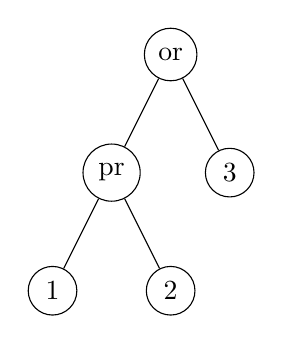
\begin{tikzpicture}
            \node [circle,draw] (z){$\orEff$}
                child { 
                    node [circle,draw] (a) {$\prEff$}
                    child { node[circle,draw] (b) {$1$} } 
                    child { node[circle,draw] (c) {$2$} }
                }
                child {
                    node [circle,draw] (d) {$3$}    
                };
        \end{tikzpicture}
        \hspace{2em}
        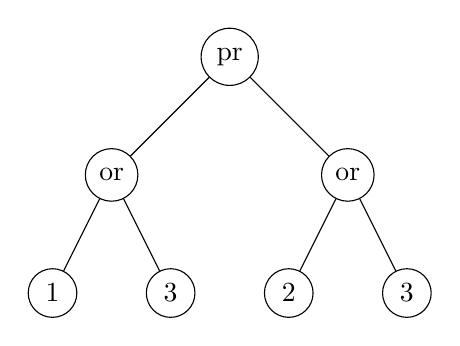
\begin{tikzpicture}[level 1/.style={sibling distance=3cm},
                            level 2/.style={sibling distance=1.5cm}]
            \node [circle,draw] (z){$\prEff$}
                child { 
                    node [circle,draw] (h) {$\orEff$}
                    child { node[circle,draw] (b) {$1$} } 
                    child { node[circle,draw] (c) {$3$} }
                }
                child {
                    node [circle,draw] (g) {$\orEff$}
                    child { node[circle,draw] (e) {$2$} } 
                    child { node[circle,draw] (f) {$3$} }
                };
        \end{tikzpicture}
    \end{center}
    \end{ensps}
    \begin{equation*}
        \orEff (\prEff (1,2), 3) \quad \quad \prEff (\orEff (1,3), \orEff (2,3))
    \end{equation*}
    \caption{The two trees from the counter example}
    \label{fig:counterexampletree}
\end{figure}

\begin{ensps}
We can see that the two trees in Figure \ref{fig:counterexampletree} 
have the same interpretation in terms of characteristic functions,
and the result from \cite{Mislove2000} shows us that a reasonable 
preorder shouldn't equate them. But we have an explicit 
cost function that shows that the interpretation in terms of 
expectancies is diffirent for the two trees:

\begin{equation*}
    h (i) = \begin{cases}
        1 & \text{ when } i = 1 \\
        8 & \text{ when } i = 2 \\
        2 & \text{ when } i = 3 \\
        0 & \text{ otherwise } 
    \end{cases}
\end{equation*}

This function can distinguish between the two trees 
because the least expected cost for the first one is $1/4$
where the least expected cost for the second one is $3/16$.

The choice of costs for $h$ is not random: we can divide 
everything by $8$ and build an actual substitution $\sigma$
such that $t_1 \sigma \not \equiv_{b} t_2 \sigma$, thus 
having an effective counter-example for the compositionality 
of the preorder.
\end{ensps}

Therefore,
this shows that for this preorder, \emph{compositionality
does not hold anymore}, even though 
it is still admissible. From a domain theoretic perspecitve,
we do have an embedding-projection pair with the domain 
of previsions using general functions, but the embedding 
is \emph{not} a homomorphism. Note that the exact same trees can be used 
as a counter example for the same claim in the case of angelic non-determinism. 


%\newpage

\section{Conclusion and future work}

The first part of this paper was about extending the results 
of Alex Simpson, Patricia Johann and Janis Voigtländer \cite{gom}
to a call-by-value setting. By doing so, some properties of 
the basic preorder $\sqeq_b$ were developed and a direct link
to denotational semantics has been made. This is a first step 
in a better understanding of basic preorders and the generality 
of the method itself. 

Some generic theorems and sanity checks have been proven 
abstractly for the logical relation and the contextual preorder
arising from $\sqeq_b$, allowing to decline them with any 
effect signature $\Sigma$. 

The ability to automatically build free preorders for an equational 
theory $\mathcal{T}$ was studied, and compared to the operational 
and denotational method in the case of probability, non-determinism
and the combination of both, showing how robust this general setting 
is.

\vspace{1em}

Obviously, the study of the requirements for a basic preorder 
are not enough, and it would be interesting to see how far we 
can weaken the admissibility property and still get results.
For instance, countable non-determinism [CIT] does \emph{not} have 
this admissibility property, but is believed to still fit in 
our setting. On the other side of the requirements, compositionality 
could be better understood using sets of observations as done in 
\cite{gom} or looking at the continuity properties of the 
monadic multiplication on trees.

It would then be interesting to try and generalise the class of 
effects, be it by adding more effects known to be algebraic, 
or blatantly non algebraic effects such as exception handling 
that would require changing the language itself, but still 
be captured by the same general method.

This work can be extended to a richer type system in the obvious 
way, and even recursive types are not an issue using step-indexing 
techniques [CITE] or by defining the projections in the language [CITE].

It could be interesting to generalise the notion of $\top\top$-closure 
to metric relations 
and talk about the distance of terms, see the work of Ugo and Raphaëlle
(and more)

Finally, the study of mixed non-determinism and probability is 
done very briefly in this paper, and there would be a lot more 
to talk about. For instance, how does the functional representation 
evolves when combining angelic,demonic and probability operators ?
Can our result be safely transported into a realisability world 
such as done in the work by Niels ?


\appendix

%\newpage 

\nocite{*}
\bibliographystyle{splncs03}
\bibliography{bibliographie}


%\begin{ensps}
%\newpage 

%\input{annexes/domaintheory}

%\newpage 

%\input{annexes/powerdomains}

%\newpage

%\input{annexes/powercones}

%\newpage

%\input{annexes/toptop}

%\newpage

%\input{annexes/obser}
%\end{ensps}

\end{document}
